%%%%% Main pour appeler les sat %%%%%
\documentclass[french, a4paper, 11pt, oneside]{book}

%%%%%%%%%%%%%%%%%%%%%%%%%%%%%%%%%%%%%%%%%%%%%%%%%%%%%%
%%%%%% regle la mise en page, et les chapitres %%%%%%%
%%%%%%%%%%%%%%%%%%%%%%%%%%%%%%%%%%%%%%%%%%%%%%%%%%%%%%
\usepackage{fancyhdr}
\usepackage[T1]{fontenc}
\usepackage[latin1]{inputenc}
\usepackage{ae}
\usepackage[frenchb]{babel}
\usepackage[french]{minitoc}
\usepackage[french]{varioref}
\usepackage{amssymb,amsbsy,amsfonts,amsmath,subeqnarray,eqnarray}
\usepackage{amsfonts}
\usepackage{vmargin}	% gere les marges
\usepackage{color}  % gere toute les couleurs
\usepackage{picins}
\usepackage{graphicx}
\usepackage[normalem]{ulem}
\usepackage{float}
\usepackage{chngpage} 
\usepackage{wrapfig}
\usepackage{program}
\usepackage{lettrine}
\usepackage{type1cm}
\usepackage{aeguill}

\usepackage{eclbkbox}
\usepackage{atxy}
\usepackage{array}
\usepackage[titletoc]{appendix}
\usepackage{makeidx}
\usepackage{subfigure}
\usepackage{braket}
\usepackage{hyperref}


\hypersetup{
     backref=true,    %permet d'ajouter des liens dans...
     pagebackref=true,%...les bibliographies
     hyperindex=true, %ajoute des liens dans les index.
     colorlinks=true, %colorise les liens
     breaklinks=true, %permet le retour a la ligne dans les liens trop longs
     urlcolor= blue,  %couleur des hyperliens
     linkcolor= blue, %couleur des liens internes
     bookmarks=true,  %cree des signets pour Acrobat
     bookmarksopen=true,            %si les signets Acrobat sont crees,
                                    %les afficher completement.
     pdftitle={Userguide IFDDA}, %informations apparaissant dans
     pdfauthor={Patrick C. Chaumet},     %dans les informations du document
     pdfsubject={IFDDA}          %sous Acrobat.
}



%%%%%%%%% declaration pour references comme ds revtex 4 %%%%%%%
\usepackage[numbers,super,sort&compress]{natbib}
\makeatletter \DeclareRobustCommand\onlinecite{\@onlinecite}
\def\@onlinecite#1{\begingroup\let\@cite
\NAT@citenum\citealp{#1}\endgroup} \makeatother
%%%%%%%%% change numerotation des footnotes %%%%%%%%%%%%%%%%%
\renewcommand{\thefootnote}{\roman{footnote}}

% A4wide pour elargir la page....

%%%% redefini les captions
\usepackage[small]{caption2}
\renewcommand{\captionfont}{\it \small}
\renewcommand{\captionlabelfont}{\it \bf \small}
\renewcommand{\captionlabeldelim}{ :}
\setlength{\captionmargin}{20 pt}%\captionmargin
%%%%%%%%%%%%%%%%%%%%%%%%%%%%%%%%%%%%%%%%%%%%%%%%%%%%%%
%%%%%%%%%%%%%%%%% regle des marges %%%%%%%%%%%%%%%%%%%
%%%%%%%%%%%%%%%%%%%%%%%%%%%%%%%%%%%%%%%%%%%%%%%%%%%%%%
\setmargins{25mm}{16mm}{150mm}{240mm}{10mm}{5mm}{10mm}{10mm}
%           left  top   width  height head  hsep foot  fskip
\setcounter{secnumdepth}{7}
\setcounter{tocdepth}{7}
\setcounter{minitocdepth}{2}
%\setcounter{lofdepth}{2}
%\setlength{\doublerulesep}{\arrayrulewidth} %% pour les tableaux(E)
%%%%%%%%%%%%%%%%%%%%%%%%%%%%%%%%%%%%%%%%%%%%%%%%%%%%%%%

%%%%%%%%%%%%%%%%%%%%%%%%%%%%%%%%%%%%%%%%%%%%%%%%%%%%%%
%%%%%%%%%%%%%%%%%% style de la page %%%%%%%%%%%%%%%%%%
%%%%%%%%%%%%%%%%%%%%%%%%%%%%%%%%%%%%%%%%%%%%%%%%%%%%%%
\definecolor{gris}{gray}{0.50}
\pagestyle{fancy}
\fancyhf{}
\renewcommand{\chaptermark}[1]{\markboth{#1}{}}
\renewcommand{\sectionmark}[1]{\markright{\thesection\ #1}}
\fancyhead[LE,RO]{\bfseries\thepage}
\fancyhead[LO,RE]{\bfseries\footnotesize\textcolor{gris}{\rightmark}}
%%%%%%%%%%%%%%%%%%%%%%%%%%%%%%%%%%%%%%%%%%%%%%%%%%%%

%%%%%%%%%%%%%%%%%%%%%%%%%%%%%%%%%%%%%%%%%%%%%%%%%%%%
%%%%%%%%%%%%%%% style des chapitres %%%%%%%%%%%%%%%%
%%%%%%%%%%%%%%%%%%%%%%%%%%%%%%%%%%%%%%%%%%%%%%%%%%%%
\makeatletter
\def\thickhrulefill{\leavevmode \leaders \hrule height 1ex \hfill \kern \z@}
\def\@makechapterhead#1{%
  %\vspace*{50\p@}%
  \vspace*{10\p@}%
  {\parindent \z@ \centering \reset@font
        \thickhrulefill\quad
        \scshape \@chapapp{} \thechapter
        \quad \thickhrulefill
        \par\nobreak
        \vspace*{10\p@}%
        \interlinepenalty\@M
        \hrule
        \vspace*{10\p@}%
        \Huge \bfseries #1\par\nobreak
        \par
        \vspace*{10\p@}%
        \hrule
    %\vskip 40\p@
    \vskip 100\p@
  }}
\def\@makeschapterhead#1{%
  %\vspace*{50\p@}%
  \vspace*{10\p@}%
  {\parindent \z@ \centering \reset@font
        \thickhrulefill
        \par\nobreak
        \vspace*{10\p@}%
        \interlinepenalty\@M
        \hrule
        \vspace*{10\p@}%
        \Huge \bfseries #1\par\nobreak
        \par
        \vspace*{10\p@}%
        \hrule
    %\vskip 40\p@
    \vskip 100\p@
  }}
%%%%%%%%%%%%%%%%%%%%%%%%%%%%%%%%%%%%%%%%%%%%%%%%%%%%
% L'environnement changemargin d�crit ci-dessous permet de
% modifier localement les marges d'un document. Il prend deux
% arguments, la marge gauche et la marge droite (ces arguments
% peuvent prendre des valeurs n�gatives).
%%%% debut macro %%%%
\newenvironment{changemargin}[2]{\begin{list}{}{%
\setlength{\topsep}{0pt}%
\setlength{\leftmargin}{0pt}%
\setlength{\rightmargin}{0pt}%
\setlength{\listparindent}{\parindent}%
\setlength{\itemindent}{\parindent}%
\setlength{\parsep}{0pt plus 1pt}%
\addtolength{\leftmargin}{#1}%
\addtolength{\rightmargin}{#2}%
}\item }{\end{list}}
%%%%%%%%%%%
\interfootnotelinepenalty=10000
%%%evite les orphelins
\widowpenalty=10000
\clubpenalty=10000
\raggedbottom

\lccode`\'=`\'

\hyphenation{�-lec-tro-ma-gn�-ti-que po-la-ri-sa-bi-li-t�
  dif-f�-ren-tes ma-cros-co-pi-que lo-gi-que-ment dis-cr�-ti-sa-tion
  in-ci-dent u-ni-que-ment}



%%%% fin macro %%%%
%%%%%%%%%%%%%%%%%%%%%%%%%%%%%%%%%%%%%%%%%%%%%%%%%%%%
%%%%%%%%%%%%%% Debut du document %%%%%%%%%%%%%%%%%%%
%%%%%%%%%%%%%%%%%%%%%%%%%%%%%%%%%%%%%%%%%%%%%%%%%%%%
\begin{document}
\frontmatter 
%%%%%%%%%%%%%%%%%%%%%%%%%%%%%%%%%%%%%%%%%%%%%%%%%%%%%%%%
%              Definition des variables                %
%%%%%%%%%%%%%%%%%%%%%%%%%%%%%%%%%%%%%%%%%%%%%%%%%%%%%%%%
%\newcommand{\letchap}[2]{\lettrine[nindent=10pt,loversize=0.08,lines=3,slope=-0.4em,lhang=-0.5,lraise=0.25]{#1}{#2}}
\newcommand{\letchap}[2]{\lettrine[nindent=10pt,loversize=-0.02,lines=3,slope=-0.5em,lhang=-0.5,lraise=-0.0]{#1}{#2}}
\newcommand{\ve}[1]{\boldsymbol{#1}}
%----------------------------------------
\newcommand{\beq}{\begin{equation}}
\newcommand{\eeq}{\end{equation}}
\newcommand{\nn}{\nonumber}
%----------------------------------------
\newcommand{\be}{\begin{eqnarray}}
\newcommand{\ee}{\end{eqnarray}}
%----------------------------------------
\newcommand{\bdm}{\begin{displaymath}}
\newcommand{\edm}{\end{displaymath}}
%----------------------------------------
\newcommand{\etal}{{\it et al.~}}
\newcommand{\degexp}{^{\circ}}

\newcommand{\ds}{{\rm d}S}
\newcommand{\dv}{{\rm d}V}
\newcommand{\vect}[1]{\overrightarrow{#1}}
\newcommand{\tenseur}[1]{\overleftrightarrow{#1}}
\newcommand{\grad}{\vect{\rm grad~}}
\renewcommand{\div}{{\rm div~}}
\newcommand{\rot}{\vect{\rm rot~}}
\newcommand{\benn}{\begin{eqnarray*}}
\newcommand{\eenn}{\end{eqnarray*}}
\newcommand{\prodv}{\,{_\wedge}\,}
\newcommand{\venab}{\ve{\nabla}}
\newcommand{\dl}{{\rm d}\vect{l}}
\newcommand{\quatpieps}{4\pi\varepsilon_0}
\newcommand{\covect}[1]{\vect{\underline{#1}}}
\newcommand{\phar}{ \left< {\cal{P}} \right >}
\newcommand{\pscat}{ \left< {\cal{P}}_{\rm scattered} \right >}
\newcommand{\prad}{ \left< {\cal{P}}_{\rm radiated} \right >}
\newcommand{\pext}{ \left< {\cal{P}}_{\rm extinction} \right >}
\newcommand{\pabs}{ \left< {\cal{P}}_{\rm absorbed} \right >}
\newcommand{\prem}{ \left< {\cal{P}}_{\rm extinction} \right >}
\renewcommand{\labelitemi}{$\bullet$}
\pagenumbering{roman}
%%%%%%%%%%%%%%%%%%%%%%%%%%%%%%%%%%%%%%%%%%%%%%%%%%%%%%
%%%%%%%%%%%%%%%%% PAGE DE GARDE  %%%%%%%%%%%%%%%%%%%%%
%%%%%%%%%%%%%%%%%%%%%%%%%%%%%%%%%%%%%%%%%%%%%%%%%%%%%%

%Une commande sembleble � \rlap ou \llap, mais centrant son argument
\def\clap#1{\hbox to 0pt{\hss #1\hss}}%
%Une commande centrant son contenu (� utiliser en mode vertical)
\def\ligne#1{%
  \hbox to \hsize{%
    \vbox{\centering #1}}}%
%Une comande qui met son premier argument � gauche, le second au 
%milieu et le dernier � droite, la premi�re ligne ce chacune de ces
%trois boites co�ncidant
\def\haut#1#2#3{%
  \hbox to \hsize{%
    \rlap{\vtop{\raggedright #1}}%
    \hss
    \clap{\vtop{\centering #2}}%
    \hss
    \llap{\vtop{\raggedleft #3}}}}%
%Idem, mais cette fois-ci, c'est la derni�re ligne
\def\bas#1#2#3{%
  \hbox to \hsize{%
    \rlap{\vbox{\raggedright #1}}%
    \hss
    \clap{\vbox{\centering #2}}%
    \hss
    \llap{\vbox{\raggedleft #3}}}}%
%La commande \maketitle
\def\maketitle{%
  \thispagestyle{empty}\vbox to \vsize{%
    \haut{}{\@blurb}{}
    \vspace{3cm}
   
    %\vfill
    \begin{center}\leavevmode
    	\normalfont
    	{\raggedleft \@author\par}%
    	%\thickhrulefill\par
    	\vspace{20mm} \hrule height 2pt 
    	{\huge\center \textbf{\@title}}%
    	\vspace{5mm} \hrule height 2pt \vspace{5mm}
	\vfill
    	\vskip 1cm
    	{\LARGE\center\textsc{}}
    	\vskip 2cm

    	
    \end{center}% 
    \vskip 1cm
    }%
  \cleardoublepage
  }

%Les commandes permettant de d�finir la date, le lieu, etc.
\def\date#1{\def\@date{#1}}
\def\author#1{\def\@author{#1}}
\def\title#1{\def\@title{#1}}
\def\location#1{\def\@location{#1}}
\def\blurb#1{\def\@blurb{#1}}
\def\email#1{\def\@email{#1}}
%Valeurs par d�faut
\date{\today}
\author{}
\title{}
\location{Marseille}
\blurb{}
\email{patrick.chaumet@fresnel.fr}
\makeatother
%
%%%%%%%%%%%%%%%%%%%%%%%%%%%%%%%%%%%%%%%%%%%%%%%%%%%%%%%%%%%%%%%%%%%%
\blurb{
\begin{center}
\parpic{
%\resizebox{160mm}{!}{\includegraphics{logofac.eps}}
}
\picskip{0}
\end{center}
 {\huge \textsc{Institut Fresnel}} 
}

\title{IF-DDA \\ \vspace{5mm} \textsc{Idiot Friendly-Discrete Dipole
    Approximation}\\ \vspace{5mm} {\Large version : 0.6.5} }
\author{\center{\LARGE \textsc{Patrick
      C. Chaumet} \\ \vspace{5mm} \textsc{Daniel Sentenac} \\
    \vspace{5mm} \textsc{Anne Sentenac}}}

\atxy(3cm,17cm){\resizebox{140mm}{!}{\includegraphics{schemamic.eps}}}



\email{patrick.chaumet@fresnel.fr}
\date{}


\newpage{\pagestyle{empty}\cleardoublepage}


\maketitle
\newpage{\pagestyle{empty}\cleardoublepage}
\newpage{\pagestyle{empty}\cleardoublepage}
\dominitoc 
\newpage{\pagestyle{empty}\cleardoublepage}
\tableofcontents
\clearpage{\pagestyle{empty}\cleardoublepage}
\addstarredchapter{Liste des figures}
\listoffigures
\clearpage{\pagestyle{empty}\cleardoublepage}
%\include{remerciements}
\mainmatter 
\pagenumbering{arabic}
\chapter{G�n�ralit�s}\label{chap1}
\markboth{\uppercase{G�n�ralit�s}}{\uppercase{G�n�ralit�s}}

\minitoc

\section{Introduction}


Ce logiciel permet de calculer la diffraction d'une onde
�lectromagn�tique par un objet tridimensionnel. Cette interaction est
prise en compte rigoureusement par la r�solution des �quations de
Maxwell, mais peut aussi le faire par des m�thodes approch�es telles
que l'approximation de Born � l'ordre 0 ou 1. Le code par une
interface conviviale permet de choisir des objets canoniques (sph�re,
cube,,cylindre , sph�res concentriques, ...) ainsi que des ondes
incidentes pr�d�finies (onde plane, faisceau Gaussien, speckle,...)
ainsi que des objets et incidents arbitraires. Apr�s par des menus
d�roulants, il est facile d'�tudier les sections efficaces, la
diffraction champ proche et champ lointain ainsi que la microscopie.


A noter qu'il existe de nombreuses m�thodes permettant d'�tudier la
diffraction d'une onde �lectromagn�tique par un objet de forme et de
permittivit� relative arbitraires. Nous n'allons par faire ici une
liste exhaustive de ces m�thodes, mais le lecteur int�ress� peut se
reporter � l'article de F. M. Kahnert qui d�taille les forces et les
faiblesses des m�thodes les plus usuelles.~\cite{Kahnert_JQSRT_03}

La m�thode que nous utilisons s'appelle la m�thode des dip�les coupl�s
(CDM) ou dip�le discret approximation (DDA). Cette m�thode, dite
volumique car le champ diffract� est obtenu � partir d'une int�grale
dont le support est le volume de l'objet consid�r�, a �t� introduite
par E. M. Purcell et C. R. Pennypacker en 1973 pour �tudier la
diffusion de la lumi�re par des grains dans le milieu
interstellaire.~\cite{Purcell_AJ_73}

\section{Le principe de la DDA}\label{paprincipecdm}

Nous pr�sentons dans ce paragraphe la DDA d'une mani�re volontairement
simpliste. Soit un objet de forme et de permittivit� relative
arbitraires dans syst�me multicouche. Cet objet en pr�sence du
multicouche est soumis � une onde �lectromagn�tique incidente de
longueur d'onde $\lambda$ ($k_0=2\pi/\lambda$). Le principe de la DDA
consiste � repr�senter l'objet en un ensemble de $N$ petits cubes
d'ar�te $a$ [par petits, nous entendons plus petits que la longueur
  d'onde dans l'objet : $a\ll \lambda/\sqrt{\varepsilon}$
  (Fig.~\ref{discretisation})].
%%%%%%%%%%%%%%%%%%%%%%%%%%%%%%%%%%%%%%%%%%%%%%%%%%%%%%%%%%%%%%%%%%%%%%
\begin{figure}
\begin{center}
\includegraphics*[draft=false,width=150mm]{discretisation.eps}
\caption{Principe de la DDA : l'objet � �tudier (� gauche) est
 discr�tis� en un ensemble de petits dip�les (� droite).}
\label{discretisation}
\end{center}
\end{figure}
%%%%%%%%%%%%%%%%%%%%%%%%%%%%%%%%%%%%%%%%%%%%%%%%%%%%%%%%%%%%%%%%%%%%%%
Chacun des petits cubes sous l'action de l'onde incidente va se
polariser, et donc acqu�rir un moment dipolaire, dont la valeur va
d�pendre du champ incident, de son interaction avec ses voisins et
avec les interfaces du syst�me. Le champ local � la position d'un
dip�le localis� en $\ve{r}_i$, $\ve{E}(\ve{r}_i)$ est la somme du
champ de r�f�rence plus du champ rayonn� par les $N$ dip�les :
%%%%%%%%%%%%%%%%%%%%%%%%%%%%%%%%%%%%%%%%%%%%%%%%%%%%%%%%%%%%%%%%%%%%%%
\be \label{cdms} \ve{E}(\ve{r}_i)=\ve{E}_{\rm
  ref}(\ve{r}_i)+\sum_{j=1}^{N}
\ve{G}(\ve{r}_i,\ve{r}_j)\alpha(\ve{r}_j)\ve{E}(\ve{r}_j). \ee
%%%%%%%%%%%%%%%%%%%%%%%%%%%%%%%%%%%%%%%%%%%%%%%%%%%%%%%%%%%%%%%%%%%%%%
$\ve{E}_{\rm ref}$ est le champ de r�f�rence, $\ve{G}$ la
susceptibilit� lin�aire du champ d'un multicouche.  $\alpha$ est la
polarisabilit� de chaque �l�ment de discr�tisation obtenue � partir de
la relation de Claussius-Mossotti. Notons que la polarisabilit�
$\alpha$, pour respecter le th�or�me optique, se doit de contenir un
terme dit de r�action de rayonnement.~\cite{Draine_AJ_88}
L'Eq.~(\ref{cdms}) est vraie pour $i=1,\cdots,N$, et repr�sente donc
un syst�me de $3N$ �quations lin�aires � r�soudre, les champs locaux,
$\ve{E}(\ve{r}_i)$, �tant les inconnus. Une fois le syst�me
d'�quations lin�aires r�solu, le champ diffus� par l'objet � une
position $\ve{r}$ arbitraire, est obtenu en faisant la somme de tous
les champs rayonn�s par chacun des dip�les :
%%%%%%%%%%%%%%%%%%%%%%%%%%%%%%%%%%%%%%%%%%%%%%%%%%%%%%%%%%%%%%%%%%%%%%
\be \label{cdmd} \ve{E}(\ve{r})=\sum_{j=1}^{N} \ve{G}(\ve{r},\ve{r}_j)
\alpha(\ve{r}_j) \ve{E}(\ve{r}_j). \ee
%%%%%%%%%%%%%%%%%%%%%%%%%%%%%%%%%%%%%%%%%%%%%%%%%%%%%%%%%%%%%%%%%%%%%%
Nous venons de pr�senter la DDA telle que l'ont pr�sent�e E. M.
Purcell and C. R. Pennypacker.~\cite{Purcell_AJ_73} Notons qu'une
autre m�thode tr�s proche de la DDA existe. Cette m�thode, dite
m�thode des moments, part de l'�quation int�grale de Lippman
Schwinger, est, moyennant quelques hypoth�ses, strictement identique �
la DDA. La d�monstration de l'�quivalence entre ces deux m�thodes
�tant un peu technique, elle est explicit�e dans la
Ref.~\onlinecite{Chaumet_PRE_04}.

Les avantages de la DDA sont qu'elle est applicable � des objets de
forme arbitraire, inhomog�ne (chose difficilement r�alisable dans le
cas de m�thode surfacique), et anisotrope (la polarisabilit� associ�e
aux �l�ments de discr�tisation devient alors tensorielle). La
condition d'onde sortante est automatiquement satisfaite � travers la
susceptibilit� lin�aire du champ. Notons enfin, que seul l'objet est
discr�tis�, contrairement aux m�thodes de diff�rences finies et
�l�ments finis.~\cite{Kahnert_JQSRT_03}

L'inconv�nient majeur de la DDA consiste en une croissance rapide du
temps de calcul avec l'augmentation du nombre d'�l�ments de
discr�tisation, {\it i.e.}, l'augmentation de la taille du syst�me
d'�quations lin�aires � r�soudre. Il existe des moyens pour acc�l�rer
la r�solution d'un syst�me d'�quations lin�aires de tr�s grande
taille, telle que la m�thode des gradients conjugu�s, mais malgr�
tout, des valeurs de $N>10^6$ en espace homog�ne sont difficiles �
traiter.


\section{Un mot sur le code}

Le code est pens� pour avoir une interface conviviale afin que tout le
monde puisse l'utiliser sans probl�me y compris des non
sp�cialistes. Ceci permet alors � des �tudiants de premier cycle
d'�tudier par exemple les bases de la microscopie (crit�re de
Rayleigh, notion d'ouverture num�rique,...) ou de la diffraction sans
aucun probl�me; et � des chercheurs, typiquement des biologistes,
n'ayant aucune notion des �quations de Maxwell de simuler ce que donne
un microscope (brightfield, microscope de phase, champ sombre,...) en
fonction des param�tres usuels et de l'objet. N�anmoins, ce code peut
aussi servir � des physiciens sp�cialistes de l'�lectromagn�tisme �
travers, par exemple, de calculs de forces optiques, de diffraction,
de sections efficaces, de champ proche et ceci avec de nombreux types
de faisceaux incidents et diff�rentes m�thodes de calculs du champ
�lectromagn�tique.

Le code pr�sente donc par d�faut une interface simple ou tous les
d�tails num�riques sont cach�s et o� de nombreuses options sont alors
choisies par d�faut. Mais il est facile d'acc�der � tous les
possibilit�s de code en cochant l'option interface avanc�e. Ce guide
utilisateur explique le fonctionnement de l'interface avanc�e en
commen�ant par les diff�rents approches utilis�es par le code pour
r�soudre les �quations de Maxwell.

A noter que la convivialit� du code est faite au d�triment de
l'optimisation de la RAM et le code peut donc �tre gourmand en m�moire
pour les gros objets.


\section{Comment compiler le code}
Pour faire tourner le code sur un syst�me linux il est n�cessaire
d'avoir install� les paquets suivants: qt, qt-devel, gcc-c++ et
gfortran. Noter qu'il y a trois versions du code, la premi�re en
s�quentielle qui utilise FFT singleton, la deuxi�me en parall�le et
qui utilise FFTW (Fast Fourier Transform in the west) et qui n�cessite
openmp version 4.5 minimum, et la troisi�me qui utilise en plus le
format HDF5 pour sauvegarder les donn�es dans un seul fichier
binaire. Par d�faut le code est compil� sans HDF5 et FFTW ce qui donne
donc un code avec des FFT plus lentes et qui n'est pas parall�lis� et
une �criture des datas forc�ment en ascii. Actuellement selon l'age du
linux que vous utilisez vous avez Qt4 ou Qt5. Le code a �t� test� sous
les deux environnements par contre pour compiler il faut bien s�r
s'adpater qt4 devenant qt5 sur les versions r�centes, je noterai pour
faire compact qt4(5).


\begin{tabular}{|c|c|c|}
  \hline
  Code par d�faut & Code avec FFTW & Code avec FFTW et HDF5 \\
  \hline
  qmake-qt4(5) & qmake-qt4(5) ``CONFIG+=fftw'' & qmake-qt4(5) ``CONFIG+=fftw hdf5'' \\
  make & make & make \\
make install & make install & make install \\
  \hline
\end{tabular}
Puis pour lancer le code, taper, cd bin, puis ./cdm.



Sur linux la version avec FFTW n�cessite d'installer les packages FFTW
avec par exemple ``dnf install *fftw*''. Pour la version qui utilise
en plus HDF5 il faut installer en plus les packages suivant ``dnf
install hdf hdf5 hdf5-static hdf5-devel''.


Si on veut utiliser le code sans interface graphique, c'est possible
il faut alors dans le directory tests dans lequel il y a trois
``script shell''. Suivant les paquets install�s on peut alors lancer
./comp (sans FFTW et sans HDF5) ou ./compfftw (sans HDF5) ou
./compfftwhdf5. Attention suivant la configuration de votre ordinateur
peut �tre lancer avant le code un ``ulimit -s unlimited'' pour ne pas
avoir de probl�me avec la ``stacksize''. Il se cr�e donc quatre
ex�cutables dans chaun des directories test, correspondant chacun �
une configuration. SI on veut changer une donn�e il convient bien s�r
d'�diter mainsurf.f et de changer les options directement dans le code
fortran.


Le code s'installe aussi sous windows, mais la version parall�le
n�cessite �videmment d'installer FFTW sur windows.

\section{Un mot sur les auteurs}

\begin{itemize}
\item P. C. Chaumet est professeur des universit�s � l'Institut
  Fresnel de l'Universit� d'Aix-Marseille et s'occupe du d�veloppement
  du code source fortran et de l'interface.
\item A. Sentenac est directrice de recherche au CNRS et travaille �
  l'Institut Fresnel de l'Universit� d'Aix-Marseille et participe au
  d�veloppement du code sur ce qui est li� � la diffraction champ
  lointain et la microscopie.
\item D. Sentenac de l'European Gravitational Observatory en Italie
  d�veloppe l'interface conviviale du code en C++ et Qt.
\item G. Henry � l'Institut Fresnel de l'Universit� d'Aix-Marseille
  travaille sur la partie compilation du code (Ubuntu, Fedora, etc).
\end{itemize}



\section{Un mot sur la licence}


La licence est non commerciale : ShareAlike 4.0 International 4.0
International (CC BY-NC-SA 4.0)

Vous �tes libre de:

\begin{itemize}
\item partager, copier et redistribuer.
\item adapter, changer et construire dessus.
\end{itemize}


Vous devez sous cette licence suivre les conditions suivantes:
\begin{itemize}
\item Attribution - Vous devez citer les auteurs en cas d'utilisation
  du code et indiquer si des changements ont �t� faits.
\item NonCommercial - Vous ne pouvez pas utiliser le code dans un but
  commercial.
\item ShareAlike - Si vous transformer le code ou l'utilisez dans
  d'autres codes vous devez citer les auteurs et distribuez votre
  contribution sous la m�me licence que l'original.
\end{itemize}

A noter que le code est donn� sans garanti

\section{Comment citer le code}

\begin{itemize}

\item P. C. {\textsc{Chaumet}}, A. {\textsc{Sentenac}}, and
  A. {\textsc{Rahmani}}, \\{\it Coupled dipole method for scatterers
    with large permittivity.}\\ Phys. Rev. E {\bf 70}, 036606 (2004).

\item S. {\textsc{Khadir}}, P. C. {\textsc{Chaumet}},
  G. {\textsc{Baffou}} and A. {\textsc{Sentenac}}, \\{\it Quantitative
    model of the image of a radiating dipole through a
    microscope.}\\ J. Opt. Soc. Am. A {\bf 36}, 478 (2019).

\end{itemize}
   %    Generalites 
\chapter{M�thodes approch�es}\label{chapapprox}
\markboth{\uppercase{M�thodes approch�es}}{\uppercase{M�thodes approch�es}}

\minitoc

\section{Introduction}

Dans le chapitre pr�c�dent nous avons pr�sent� la DDA par une approche
simplifi� o� l'objet est un ensemble de petits dip�les rayonnant. Dans
une approche plus rigoureuse nous partons des �quations de Maxwell en
unit� Gaussienne:
%%%%%%%%%%%%%%%%%%%%%%%%%%%%%%%%%%%%%%%%%%%%%%%%%%
\be \venab \times \ve{E}^{\rm m}(\ve{r}) & = & i \frac{\omega}{c}
\ve{B}(\ve{r}) \\
\venab \times \ve{B}(\ve{r}) & = & -i \frac{\omega}{c}
\varepsilon(\ve{r}) \ve{E}^{\rm m}(\ve{r}), \ee
%%%%%%%%%%%%%%%%%%%%%%%%%%%%%%%%%%%%%%%%%%%%%%%%%%
o� $\varepsilon(\ve{r})$ est la permittivit� relative de l'objet et
$\ve{E}^{\rm m}$ le champ total dans l'objet. Ce qui nous donne
l'�quation de propagation suivante pour le champ �lectrique:
%%%%%%%%%%%%%%%%%%%%%%%%%%%%%%%%%%%%%%%%%%%%%%%%%%
\be \venab \times ( \venab \times \ve{E}^{\rm m}(\ve{r}) ) & = &
\varepsilon(\ve{r}) k_0^2 \ve{E}^{\rm m}(\ve{r}), \ee 
%%%%%%%%%%%%%%%%%%%%%%%%%%%%%%%%%%%%%%%%%%%%%%%%%%
avec $k_0=\omega^2/c^2$. En utilisant la relation
$\varepsilon=\varepsilon_{\rm mul}+4\pi \chi$ avec $\chi$ la
susceptibilit� lin�aire �lectrique, $\varepsilon_{\rm mul}$ �tant la
permittivit� relative du multicouche qui ne d�pend que de $z$, nous
avons:
%%%%%%%%%%%%%%%%%%%%%%%%%%%%%%%%%%%%%%%%%%%%%%%%%%
\be \venab \times ( \venab \times \ve{E}^{\rm m}(\ve{r}) )
-\varepsilon_{\rm mul} k_0^2 \ve{E}^{\rm m}(\ve{r}) & = & 4\pi
\chi(\ve{r}) k_0^2 \ve{E}^{\rm m}(\ve{r}) . \label{champref}\ee
%%%%%%%%%%%%%%%%%%%%%%%%%%%%%%%%%%%%%%%%%%%%%%%%%%
La solution de cette �quation sans second membre est le champ de
r�f�rence et correspond donc au milieu de r�f�rence, c'est � dire le
milieu en l'absence de l'objet �tudi� ($\chi=0$), dans notre cas le
multicouche.  Pour r�soudre cette �quation avec second membre on
cherche la fonction de Green solution de
%%%%%%%%%%%%%%%%%%%%%%%%%%%%%%%%%%%%%%%%%%%%%%%%%%
\be \venab \times ( \venab \times \ve{G}(\ve{r},\ve{r}') )
-\varepsilon_{\rm mul} k_0^2 \ve{G}(\ve{r},\ve{r}') & = & 4\pi k_0^2
\ve{I} \delta(\ve{r}-\ve{r}'), \ee
%%%%%%%%%%%%%%%%%%%%%%%%%%%%%%%%%%%%%%%%%%%%%%%%%%
La solution finale est donc:
%%%%%%%%%%%%%%%%%%%%%%%%%%%%%%%%%%%%%%%%%%%%%%%%%%
\be\ve{E}^{\rm m}(\ve{r}) = \ve{E}_{\rm ref}(\ve{r}) +\int_{\Omega}
\ve{G}(\ve{r},\ve{r}') \chi(\ve{r}') \ve{E}^{\rm m}(\ve{r}') {\rm d}
\ve{r}',\ee
%%%%%%%%%%%%%%%%%%%%%%%%%%%%%%%%%%%%%%%%%%%%%%%%%%
avec $\ve{E}_{\rm ref}$ le champ de r�f�rence solution de
l'Eq.~(\ref{champref}) sans second membre et $\Omega$ le volume
correspondant au support de l'objet �tudi�. Quand on r�sout l'�quation
dans l'objet, le champ total correspond donc au champ macroscopique
dans l'objet. Pour r�soudre cette �quation on discr�tise l'objet en un
ensemble de $N$ �l�ments de forme cubique ayant une ar�te de taille
$d$ et l'int�grale $\Omega$ sur l'objet est donc d�compos�e en une
somme d'int�grale sur chacun des �l�ments de discr�tisation de volume
$V_j=d^3$:
%%%%%%%%%%%%%%%%%%%%%%%%%%%%%%%%%%%%%%%%%%%%%%%%%%
\be\ve{E}^{\rm m}(\ve{r}_i) = \ve{E}_{\rm ref}(\ve{r}_i)
+\sum_{j=1}^{N} \int_{V_j} \ve{G}(\ve{r}_i,\ve{r}') \chi(\ve{r}')
\ve{E}^{\rm m}(\ve{r}') {\rm d} \ve{r}',\ee
%%%%%%%%%%%%%%%%%%%%%%%%%%%%%%%%%%%%%%%%%%%%%%%%%%
En supposant le champ, la fonction Green et la permittivit� constants
dans la maille, nous obtenons:
%%%%%%%%%%%%%%%%%%%%%%%%%%%%%%%%%%%%%%%%%%%%%%%%%%
\be\ve{E}^{\rm m}(\ve{r}_i) = \ve{E}_{\rm ref}(\ve{r}_i) +\sum_{j=1}^N
\ve{G}(\ve{r}_i,\ve{r}_j) \chi(\ve{r}_j) \ve{E}^{\rm m}(\ve{r}_j)
d^3.\ee
%%%%%%%%%%%%%%%%%%%%%%%%%%%%%%%%%%%%%%%%%%%%%%%%%%
Le tenseur de Green peut �tre coup� en deux parties,
$\ve{G}=\ve{M}+\ve{T}$, avec $\ve{M}$ le tenseur de Green qui prend en
compte les r�flexions multiple entre les diff�rentes interfaces et
$\ve{T}$ le tenseur de Green de l'espace homog�ne.  En utilisant, en
premi�re approximation (c'est � dire que la r�action de rayonnement
est n�glig�e, mais la prendre en compte ne changerait pas les
raisonnements qui suivent), le fait que que
$\int_{V_i}\ve{T}(\ve{r}_i,\ve{r}') {\rm d} \ve{r}'=
-4\pi/(3\varepsilon_{\rm mul}(\ve{r}_i)) $, voir
Ref.~\onlinecite{Yaghjian_PIEEE_80}) pour plus de d�tails, nous avons:
%%%%%%%%%%%%%%%%%%%%%%%%%%%%%%%%%%%%%%%%%%%%%%%%%%
\be\ve{E}^{\rm m}(\ve{r}_i) = \ve{E}_{\rm ref}(\ve{r}_i) +\sum_{j=1}^N
\ve{G}'(\ve{r}_i,\ve{r}_j) \chi(\ve{r}_j) d^3 \ve{E}^{\rm
  m}(\ve{r}_j)-\frac{4\pi}{3\varepsilon_{\rm
    mul}(\ve{r}_i)}\chi(\ve{r}_i) \ve{E}^{\rm m}(\ve{r}_i),\ee
%%%%%%%%%%%%%%%%%%%%%%%%%%%%%%%%%%%%%%%%%%%%%%%%%%
avec $\ve{G}'=\ve{M}+\ve{T}$ pour $i \neq j$ et $\ve{G}'=\ve{M}$ pour
$i=j$, et en passant toutes les d�pendances en $i$ � gauche de la relation
nous avons au final:
%%%%%%%%%%%%%%%%%%%%%%%%%%%%%%%%%%%%%%%%%%%%%%%%%%
\be\ve{E}(\ve{r}_i) & = & \ve{E}_{\rm ref}(\ve{r}_i) +\sum_{j=1}^N
\ve{G}'(\ve{r}_i,\ve{r}_j) \alpha_{\rm CM}(\ve{r}_j) \ve{E}(\ve{r}_j)
\\ {\rm with} \phantom{000} \ve{E}(\ve{r}_i) & = &
\frac{\varepsilon(\ve{r}_i)+2\varepsilon_{\rm
    mul}(\ve{r}_i)}{3\varepsilon_{\rm mul}(\ve{r}_i)} \ve{E}^{\rm
  m}(\ve{r}_i) \\ \alpha_{\rm CM}(\ve{r}_j) & = & \frac{3}{4\pi}
\varepsilon_{\rm mul}(\ve{r}_i) d^3
\frac{\varepsilon(\ve{r}_i)-\varepsilon_{\rm
    mul}(\ve{r}_i)}{\varepsilon(\ve{r}_i)+2\varepsilon_{\rm
    mul}(\ve{r}_i)} .\ee
%%%%%%%%%%%%%%%%%%%%%%%%%%%%%%%%%%%%%%%%%%%%%%%%%%
Le champ $\ve{E}(\ve{r}_i)$ est le champ local, c'est � dire que c'est
le champ dans la maille $i$ en l'absence de la maille elle m�me. En
�crivant cette �quation pour toutes les valeurs de $i$ nous avons un
syst�me d'�quations lin�aires que nous pouvons �crire symboliquement
comme:
%%%%%%%%%%%%%%%%%%%%%%%%%%%%%%%%%%%%%%%%%%%%%%%%%%
\be \ve{E} = \ve{E}_{\rm ref} + \ve{A} \ve{D}_\alpha \ve{E},\ee
%%%%%%%%%%%%%%%%%%%%%%%%%%%%%%%%%%%%%%%%%%%%%%%%%%
avec $\ve{A}$ qui contient toutes les fonctions de Green et
$\ve{D}_\alpha$ une matrice diagonale qui contient toutes les
polarisabilit�s de chaque �l�ment de discr�tisation. Nous d�taillons
au chapitre suivant comment r�soudre rigoureusement ce syst�me
d'�quation lin�aire, mais dans ce pr�sent chapitre nous d�taillons les
diff�rentes approches possibles pour �viter la r�solution du syst�me
qui est tr�s gourmande en temps de calcul.

A noter que le champ diffract� par l'objet en dehors du support de
l'objet s'�crit simplement comme:
%%%%%%%%%%%%%%%%%%%%%%%%%%%%%%%%%%%%%%%%%%%%%%%%%%
\be\ve{E}^{\rm d}(\ve{r}) & = & \sum_{j=1}^N \ve{G}(\ve{r},\ve{r}_j)
\alpha(\ve{r}_j) \ve{E}(\ve{r}_j). \ee
%%%%%%%%%%%%%%%%%%%%%%%%%%%%%%%%%%%%%%%%%%%%%%%%%%



\section{Les diff�rentes m�thodes approch�es utilis�es dans le code}


\subsection{Born}


Une approximation simple est l'approximation de Born, c'est � dire que
le champ macroscopique dans l'objet est le champ incident. Nous avons
donc :
%%%%%%%%%%%%%%%%%%%%%%%%%%%%%%%%%%%%%%%%%%%%%%%%%%
\be \ve{E}^{\rm m}(\ve{r}_i) = \ve{E}_{\rm ref}(\ve{r}_i), \ee
%%%%%%%%%%%%%%%%%%%%%%%%%%%%%%%%%%%%%%%%%%%%%%%%%%
pour tous les �l�ments de discr�tisation. Apr�s il suffit de faire
propager le champ. Il est �vident que cette approximation tient si le
contraste et la taille de l'objet sont petits.


\subsection{Born renormalis�}

Nous pouvons faire l'hypoth�se � l'identique mais sur le champ local,
c'est � dire que :
%%%%%%%%%%%%%%%%%%%%%%%%%%%%%%%%%%%%%%%%%%%%%%%%%%
\be \ve{E}(\ve{r}_i) = \ve{E}_{\rm ref}(\ve{r}_i). \ee
%%%%%%%%%%%%%%%%%%%%%%%%%%%%%%%%%%%%%%%%%%%%%%%%%%
En consid�rant la relation entre le champ local et le champ
macroscopique nous avons alors:
%%%%%%%%%%%%%%%%%%%%%%%%%%%%%%%%%%%%%%%%%%%%%%%%%%
\be  \ve{E}^{\rm m}(\ve{r}_i) = \frac{3}{\varepsilon(\ve{r}_i)+2}
\ve{E}_{\rm ref}(\ve{r}_i). \ee
%%%%%%%%%%%%%%%%%%%%%%%%%%%%%%%%%%%%%%%%%%%%%%%%%%
La phase est la m�me que dans le cas de l'approximation de Born mais
l'amplitude est chang�e. Cette approximation est meilleure pour des
permittivit�s plus fortes car fait une correction sur l'amplitude du
champ macroscopique, nous avons appel� cette approximation Born
renormalis�.


\subsection{Born � l'ordre 1}

Sans r�soudre le syst�me d'�quations lin�aires on peut faire un Born
renormalis� � l'ordre 1, c'est � dire que l'on effectue:
%%%%%%%%%%%%%%%%%%%%%%%%%%%%%%%%%%%%%%%%%%%%%%%%%%
\be\ve{E}(\ve{r}_i) & = & \ve{E}_{\rm ref}(\ve{r}_i) +\sum_{j=1}^N
\ve{G}'(\ve{r}_i,\ve{r}_j) \alpha(\ve{r}_j) \ve{E}_{\rm
  ref}(\ve{r}_j). \ee
%%%%%%%%%%%%%%%%%%%%%%%%%%%%%%%%%%%%%%%%%%%%%%%%%%
Ceci permet de prendre en compte un peu la variation du champ dans
l'objet et permet de traiter des objets plus grands mais toujours avec
un contraste faible. Il est possible de d�velopper Born � des ordres
sup�rieurs mais quand le contraste devient fort la s�rie ne converge
plus...

\section{Calcul des fonctions de Green}

Bien que nous utilisions une m�thode tr�s efficace de calcul du
tenseur de Green, voir Ref.~\onlinecite{Paulus_PRE_00}, cela prend
quand m�me du temps d'�valuer toutes les couples observations dip�les
constituant l'objet. Pour acc�l�rer le calcul nous allons utiliser
l'invariance translationelle dans le plan $(x,y)$ du syst�me
multicouche, soit
$\ve{G}(\ve{r},\ve{r}')=\ve{G}(\|\ve{r}_{\parallel}-\ve{r}_{\parallel}'\|,z,z')$. Pour
chaque couple $(z,z')$, le nombre de tenseur de Green � �valuer pour
tous les distances dans le plan $(x,y)$ avec un maillage de
$ n_x \times n_y$ avec $n_x>n_y$ est �gal � $n_y(2 n_x-n_y+1)/2$, ce
qui cro�t en $n_x^2$. Pour acc�l�rer le calcul, nous pouvons approcher
le tenseur de Green
$\ve{G}(\|\ve{r}_{\parallel}-\ve{r}_{\parallel}'\|,z,z')$ en utilisant
une interpolation sur un ensemble de points tels que
$\ve{G}(qd/n_d,z,z')$ avec $q=1,\cdots, {\rm int}\sqrt{ n_x^2+n_y^2}$
et $n_d$ un nombre entier. Cette fois-ci le nombre de tenseur de Green
� �valuer est proportionnel � $n_d n_x$ ce qui est beaucoup moins
gourmand en temps de calcul et tous les couples observations dip�les
sont alors estim�s par interpolation � partir du jeu de donn�e
initial.



Notons que les interpolations lin�aires ou polynomiales ne peuvent
�valuer le tenseur de Green correctement quand
$\|\ve{r}_{\parallel}-\ve{r}_{\parallel}'\|<\lambda$, du fait de la
d�croissance rapide des ondes �vanescentes. Pour obtenir une meilleure
interpolation nous avons utiliser des fonctions rationnelles qui permet
de prendre compte des p�les (Press et al. 1986) et permet une
approximation pr�cise du comportement en $1/r^3$ du tenseur de Green
dans la zone de champ proche.



Dans le code, dans la section param�tre num�rique, le menu d�roulant
Green fonction permet de choisir soit de calculer rigoureusement le
tenseur de Green, soit � partir d'interpolation plus ou moins fine
suivant la valeur de $n_d=1, 2, 3, 4$. Par d�faut la valeur $n_d=2$
est utilis�e ce qui est suffisamment pr�cis. Notons que le calcul des
tenseurs de Green par interpolation est parall�lis� ce qui n'est pas le
cas du calcul rigoureux, soit encore un gain de temps
appr�ciable.

\chapter{D�tails num�riques}\label{chappola}
\markboth{\uppercase{D�tails num�riques}}{\uppercase{D�tails
    num�riques}}

\minitoc

\section{Polarisabilit�}


Comme vu au chapitre pr�c�dent la DDA d�coupe l'objet en un ensemble
de dip�le ponctuel, o� � chaque dip�le ponctuel est associ� une
polarisabilit� $\alpha$. Il existe diff�rente forme pour cette
polarisabilit�. La premi�re a avoir �t� utilis�e, et la plus simple
qui a �t� introduite au chapitre pr�c�dent, est la relation de
Clausius Mossotti (CM)~\cite{Purcell_AJ_73}:
%%%%%%%%%%%%%%%%%%%%%%%%%%%%%%%%%%%%%%%%%%%%%%%%%%%%%%%%%
\be \alpha_{\rm CM} & = & \frac{3}{4\pi}\varepsilon_{\rm mul}
\frac{\varepsilon-\varepsilon_{\rm mul}}{\varepsilon+2\varepsilon_{\rm
    mul}}d^3= \varepsilon_{\rm mul} \frac{\varepsilon-\varepsilon_{\rm
    mul}}{\varepsilon+2\varepsilon_{\rm mul}}a^3, \ee
%%%%%%%%%%%%%%%%%%%%%%%%%%%%%%%%%%%%%%%%%%%%%%%%%%%%%%%%%
avec $\varepsilon$ la permittivit� de l'objet, $d$ la taille de la
maille cubique et $a=\left(\frac{3}{4\pi}\right)^{\frac{1}{3}}d$ qui
est le rayon de la sph�re de m�me volume que la maille cubique de c�t�
$d$ et $\varepsilon_{\rm mul}=n_{\rm mul}^2$ la permittivit� relative
de la couche.  Malheureusement cette relation ne conserve pas
l'�nergie et il faut alors introduire un terme de r�action de
rayonnement qui tient compte du fait que des charges en mouvement
perdent de l'�nergie, et la polarisabilit� s'�crit
alors~\cite{Draine_AJ_88}:
%%%%%%%%%%%%%%%%%%%%%%%%%%%%%%%%%%%%%%%%%%%%%%%%%%%%%%%%%
\be \alpha_{\rm RR} & = & \frac{\alpha_{\rm CM}}{1-\frac{2}{3} i k_0^3
  n_{\rm mul} \alpha_{\rm CM}}.  \ee
%%%%%%%%%%%%%%%%%%%%%%%%%%%%%%%%%%%%%%%%%%%%%%%%%%%%%%%%%
Apr�s diff�rentes formes de la polarisabilit� ont �t� �tablies pour
am�liorer la pr�cision de la DDA et prendre en compte le caract�re non
ponctuel dip�le, et on peut citer parmi les plus connues celles de
Goedecke et O'Brien~\cite{Goedecke_AO_88},
%%%%%%%%%%%%%%%%%%%%%%%%%%%%%%%%%%%%%%%%%%%%%%%%%%%%%%%%%
\be \alpha_{\rm GB} & = & \frac{\alpha_{\rm CM}}{1-\frac{2}{3} i k_0^3
  n_{\rm mul} \alpha_{\rm CM}-k_0^2 \alpha_{\rm CM}/a}, \ee
%%%%%%%%%%%%%%%%%%%%%%%%%%%%%%%%%%%%%%%%%%%%%%%%%%%%%%%%%
de Lakhtakia~\cite{Lakhtakia_IJMPC_92}:
%%%%%%%%%%%%%%%%%%%%%%%%%%%%%%%%%%%%%%%%%%%%%%%%%%%%%%%%%
\be \alpha_{\rm LA} & = & \frac{ \alpha_{\rm CM} }{1- 2
  \frac{\varepsilon-\varepsilon_{\rm
      mul}}{\varepsilon+2\varepsilon_{\rm mul}} \left[ (1-i k_0 n_{\rm
      mul} a)e^{i k_0 n_{\rm mul} a}-1\right] } \ee
%%%%%%%%%%%%%%%%%%%%%%%%%%%%%%%%%%%%%%%%%%%%%%%%%%%%%%%%%
et de Draine et Goodman~\cite{Draine_AJ_93}
%%%%%%%%%%%%%%%%%%%%%%%%%%%%%%%%%%%%%%%%%%%%%%%%%%%%%%%%%
\be \alpha_{\rm LR} & = & \frac{ \alpha_{\rm CM}}{ 1 + \alpha_{\rm CM}
  \left[ \frac{(b_1+\varepsilon b_2/\varepsilon_{\rm mul} +\varepsilon
      b_3/\varepsilon_{\rm mul} S)k_0^2}{d}-\frac{2}{3} i n_{\rm mul}
    k_0^3 \right] }, \ee
%%%%%%%%%%%%%%%%%%%%%%%%%%%%%%%%%%%%%%%%%%%%%%%%%%%%%%%%%
avec $b_1=-1.891531$, $b_2=0.1618469$, $b_3=-1.7700004$ et $S=1/5$.

Dans le code par d�faut c'est $\alpha_{\rm RR}$ qui est utilis�e par
d�faut. Dans le cas o� la permittivit� est anisotrope seule
$\alpha_{\rm RR}$ ou $\alpha_{\rm CM}$ seront utilis�es.


Une derni�re polarisabilit� est introduite (PS) qui ne fonctionne que
pour les sph�res homog�nes et marche particuli�rement bien pour les m�taux. 
Cela consiste � effectuer un changement de polarisabilit� des �l�ments
 sur le bord de la sph�re en prenant en compte le facteur de
 d�polarisation de la sph�re.~\cite{Rahmani_AJ_04}

\section{R�soudre le syst�me d'�quation lin�aire}

Nous avons, pour conna�tre le champ �lectrique local dans l'objet,
c'est � dire � la position des $N$ �l�ments de discr�tisation, �
r�soudre le syst�me d'�quation lin�aire suivant:
%%%%%%%%%%%%%%%%%%%%%%%%%%%%%%%%%%%%%%%%%%%%%%%%%%%%%%%%%
\be \ve{E} = \ve{E}_0 + \ve{A} \ve{D}_\alpha \ve{E},\ee
%%%%%%%%%%%%%%%%%%%%%%%%%%%%%%%%%%%%%%%%%%%%%%%%%%%%%%%%%
o� $\ve{E}_0$ est un vecteur de taille $3N$ qui contient les champs
incidents sur chacun des �l�ments de discr�tisation. $\ve{A}$ est une
matrice $3N\times 3N$ qui contient tous les tenseurs de susceptibilit�
lin�aire du champ et $\ve{D}_\alpha$ est une matrice diagonale
$3N\times 3N$, si l'objet est isotrope, ou bloc diagonal $3\times 3$
si l'objet est anisotrope. $\ve{E}$ est le vecteur $3N$ qui contient
les champs �lectriques inconnus. L'�quation est r�solue par une
m�thode it�rative non lin�aire. Le code propose de nombreuses m�thodes
it�ratives et celle qui est utilis�e par d�faut est GPBICG car la plus
efficace dans de nombreux cas~\cite{Chaumet_OL_09}. Le code s'arr�te
quand le r�sidu,
%%%%%%%%%%%%%%%%%%%%%%%%%%%%%%%%%%%%%%%%%%%%%%%%%%%%%%%%%%%%%%
\be r & = & \frac{ \|\ve{E}-\ve{A} \ve{D}_\alpha \ve{E} -\ve{E}_0\|} {
  \|\ve{E}_0 \|}, \ee
%%%%%%%%%%%%%%%%%%%%%%%%%%%%%%%%%%%%%%%%%%%%%%%%%%%%%%%%%%%%%%
est en dessous de la tol�rance donn�e par l'utilisateur. A noter que
la valeur initiale est le champ incident. $10^{-4}$ est la tol�rance
utilis�e par d�faut car c'est un bon compromis entre vitesse et
pr�cision. Ci-dessous la liste des m�thodes it�ratives propos�es:
\begin{itemize}
\item GPBICG1 : Ref.~\onlinecite{Thuthu_IMECS_09}
\item GPBICG2 : Ref.~\onlinecite{Thuthu_IMECS_09}
\item GPBICGsafe : Ref.~\onlinecite{Fujino_IMECS_12}
\item GPBICGplus : Ref.~\onlinecite{Fujino_conf_13}
\item GPBICGAR1 : Ref.~\onlinecite{Thuthu_IMECS_09}
\item GPBICGAR2 : Ref.~\onlinecite{Thuthu_IMECS_09}
\item QMRCLA : Ref.~\onlinecite{Cunha_ANM_95}
\item TFQMR : Ref.~\onlinecite{Cunha_ANM_95}
\item CG : Ref.~\onlinecite{Cunha_ANM_95}
\item BICGSTAB : Ref.~\onlinecite{Cunha_ANM_95}
\item QMRBICGSTAB1 : Ref.~\onlinecite{Chan_SIAMJSC_94}
\item QMRBICGSTAB2 : Ref.~\onlinecite{Chan_SIAMJSC_94}
\item GPBICOR : Ref.~\onlinecite{Zhao_CMA_13}
\item CORS : Ref.~\onlinecite{Carpentieri_CEI_CEIW}
\item BiCGstar-plus Ref.~\onlinecite{Fujino_WCE_15}
\end{itemize}
   %    Gestion des configurations
\chapter{Gestion des configurations}\label{chap2}
\markboth{\uppercase{Gestion des configurations}}{\uppercase{Gestion
    des configurations}}

\minitoc

\section{Introduction}


Le Code se lance par ./cdm dans le dossier bin pour une configuration
linux. Celui-ci a �t� fait pour �tre le plus convivial possible et
n�cessite donc peu d'explication pour son utilisation. N�anmoins
certaines conventions ont �t� prises et demandent � �tre explicit�es.

\section{Cr�ation et sauvegarde d'une nouvelle configuration}

Pour d�marrer un nouveau calcul, aller sur l'onglet {\it calculation}
et {\it New}. Une nouvelle configuration s'affiche avec des valeurs
par d�faut. Une fois la nouvelle configuration choisie, pour la sauver
il faut choisir de nouveau l'onglet {\it Calculation} et {\it
  Save}. On choisit alors le nom de la configuration et on peut
ajouter une courte description du calcul fait.

Une autre mani�re de sauvegarder une configuration, c'est de cliquer
directement sur le panneau de la configuration {\it Save
  configuration}. Il appara�t alors deux champs, un pour le nom de la
configuration et le deuxi�me pour sa description.

\section{Gestion des configurations}

Pour g�rer toutes les configurations choisies, il faut aller sur
l'onglet {\it Calculation} et {\it Load}. Il appara�t alors une
nouvelle fen�tre avec toutes les configurations sauv�es. Pour chaque
configuration il y a une courte description que l'utilisateur a
rentr�, la date, o� le fichier configuration a �t� sauv�, puis les
caract�ristiques principales de la configuration (longueur d'onde,
puissance, col du faisceau, objet, mat�riau, discr�tisation et
tol�rance de la m�thode it�rative).  Il suffit de cliquer sur une
configuration et de cliquer sur {\it load} pour charger une
configuration.

Le bouton {\it delete} sert a supprimer une configuration sauvegard�e
et le bouton {\it export} permet d'exporter dans un fichier (nom de la
configuration.opt) toutes les caract�ristiques de la configuration.

A noter qu'en double cliquant sur la ligne, on peut modifier le champ
description.
   %    Gestion des configurations
\chapter{Propri�t�s de l'illumination}\label{chap3}
\markboth{\uppercase{Propri�t�s de
    l'illumination}}{\uppercase{Propri�t�s de l'illumination}}

\minitoc

\section{Introduction}

Dans la section propri�t�s de l'illumination, le champ {\it
  Wavelength} permet de rentrer la longueur d'utilisation. Celle-ci se
rentre en nanom�tre. Le champ $P_0$ permet de rentrer la puissance du
faisceau laser en Watt.  Le champ $W_0$ en nanom�tre permet de rentrer
pour une onde plane le rayon du faisceau laser et pour un faisceau
Gaussien la col du faisceau. A noter que dans ce code que l'onde
incidente se propage toujours dans la direction des $z$ positifs, soit
$k_z>0$ quelque soit le type de faisceau choisi.


\section{Le type de faisceau}

\subsection{Introduction}

Il y a six faisceau pr�d�finis, leur direction de propagation est
toujours d�finie de la m�me mani�re, avec deux angles $\theta$ et
$\varphi$. Ils sont reli�s � la direction donn�e par le vecteur d'onde
de la mani�re suivante:
%%%%%%%%%%%%%%%%%%%%%%%%%%%%%%%%%%%%%%%%%%%%%
\be k_x & = & k_0 \sin \theta \cos\varphi \\
k_y & = & k_0 \sin \theta \sin\varphi \\
k_z & = & k_0 \cos \theta \ee
%%%%%%%%%%%%%%%%%%%%%%%%%%%%%%%%%%%%%%%%%%%%%
o� $\ve{k}_0=(k_x,k_y,k_z)$ est le vecteur d'onde parall�le � la
direction du faisceau incident et $k_0$ le nombre d'onde, voir
Fig.~\ref{faisceau}.
%%%%%%%%%%%%%%%%%%%%%%%%%%%%%%%%%%%%%%%%%%%%%%%
\begin{figure}[H]
\begin{center}
  \includegraphics*[width=8.0cm,draft=false]{faisceau.eps}
\end{center}
\caption{D�finition de la direction du faisceau}
\label{faisceau}
\end{figure}
%%%%%%%%%%%%%%%%%%%%%%%%%%%%%%%%%%%%%%%%%%%%%%%
Pour la polarisation on utilise le plan $(x,y)$ comme surface de
r�f�rence. Alors on peut d�finir une polarisation TM ($p$) et TE
($s$), voir Fig.~\ref{pola}, ou une polarisation suivant l'axe $x$ ou
$y$.
%%%%%%%%%%%%%%%%%%%%%%%%%%%%%%%%%%%%%%%%%%%%%%%
\begin{figure}[H]
\begin{center}
  \includegraphics*[width=8.0cm,draft=false]{pola.eps}
\end{center}
\caption{D�finition de la polarisation du faisceau.}
\label{pola}
\end{figure}
%%%%%%%%%%%%%%%%%%%%%%%%%%%%%%%%%%%%%%%%%%%%%%%
Le rep�re $(x,y,z)$ sert de r�f�rentiel absolu par rapport auquel les
diff�rents �l�ments (illumination plus objets) sont rep�r�s.  Nous
d�finissons le vecteur polarisation $\ve{s}$ correspondant � la
polarisation $TE$ et le vecteur $\ve{p}$ correspondant � $TM$ comme:
%%%%%%%%%%%%%%%%%%%%%%%%%%%%%%%%%%%%%%%%%%%%%%%
\be \ve{s} & = & \frac{\hat{\ve{z}} \times \ve{k}_0}{\| \hat{\ve{z}}
  \times \ve{k}_0\|} \\
\ve{p} & = & \frac{\ve{k}_0 \times \ve{s}}{\|\ve{k}_0 \times \ve{s}\|}
.  \ee
%%%%%%%%%%%%%%%%%%%%%%%%%%%%%%%%%%%%%%%%%%%%%%%

\subsection{Linear plane wave}

{\it Linear plane wave } est une onde plane polaris�e lin�airement. La
premi�re ligne est relative � $\theta$ et la deuxi�me � $\varphi$. La
troisi�me ligne est li�e � la polarisation, la valeur pola=1 l'onde
est polaris�e en TM et pola=0 en TE d�fini comme
$\ve{E}_0=E_p \ve{p} +E_s\ve{s}$ avec $E_p={\rm pola}$ et
$E_s=\sqrt{1-\rm {pola}^2}$.  A noter que la polarisation n'est pas
forc�ment purement en TE ou TM: soit ${\rm pola}\in[0~1]$ tel que
$E^2_{\rm TM}={\rm pola}^2E^2$ et $E^2_{\rm TE}=(1-{\rm
  pola}^2)E^2$. Nous avons donc cette valeur entre 0 et 1, mais pour
des raisons simplicit�s nous avons deux valeurs particuli�res pola=3
(2) assign�es � une polarisation pour un champ orient� tel que
$\ve{E}_0 \cdot \hat{\ve{x}} =0$ ($\ve{E_0 } \cdot \hat{\ve{y}} =0$)
sans que l'utilisateur ait � faire de calcul pour trouver la valeur de
pola.

A noter que la phase est toujours prise nulle � l'origine du rep�re,
avec ${\rm Irradiance}=P_0/S$ o� $S=\pi w_0^2$ est la surface du
faisceau et $E_0=\sqrt{2 {\rm Irradiance}/c/\varepsilon_0}$.

\subsection{Circular plane wave}

{\it Circular plane wave } est une onde plane polaris�e
circulairement. La premi�re ligne est relative � $\theta$ et la
deuxi�me � $\varphi$. La troisi�me ligne est li�e � la polarisation
que l'on peut choisir droite (1) ou gauche (-1).

A noter que la phase est prise nulle � l'origine du rep�re, avec ${\rm
  Irradiance}=P_0/S$ o� $S=\pi w_0^2$ est la surface du faisceau et
$E_0=\sqrt{2 {\rm Irradiance}/c/\varepsilon_0}$.



\subsection{Multiplane wave}

{\it Multiplane wave} consiste � choisir comme illumination
diff�rentes onde planes coh�rentes. Il faut d'abord choisir le nombre
d'onde plane d�sir�, puis pour chacune des ondes planes, il faut
choisir son incidence et sa polarisation.  Dans ce cas, il faut
choisir aussi son amplitude complexe ce qui permet de d�phaser les
ondes planes les unes par rapport aux autres. La somme de la puissance
de chacune des ondes planes est �gales � $P_0$, et chaque puissance
associ�e � une onde plane est calcul�e proportionnellement � son
amplitude. A noter que si une amplitude est nulle alors le code
s'arr�te.

\subsection{Linear Gaussian}

{\it Linear Gaussian} est une onde gaussienne polaris�e
lin�airement. La premi�re ligne est relative � $\theta$ et la deuxi�me
� $\varphi$ qui d�finissent la direction incidente du faisceau
Gaussien. La troisi�me ligne est l'angle en degr� entre le vecteur
polarisation et l'axe $x$. Si cet angle est �gale � z�ro alors la
polarisation est suivant $x$, si il est �gal � 90 alors la polarisation
est suivant $y$.

Les trois lignes suivantes permettent de fixer la position
$(x_0,y_0,z_0)$ du centre du col en nanom�tres dans le rep�re
$(x,y,z)$.

A noter que cette onde Gaussienne peut avoir un col tr�s faible, car
elle est calcul�e sans aucune approximation � travers un spectre
d'onde plane fait par FFT. La d�finition du col est la suivante, pour
un faisceau de propageant suivant l'axe $z$:\cite{Agrawal_JOSA_79}
%%%%%%%%%%%%%%%%%%%%%%%%%%%%%
\be E(x,y,0)= E_0 e^{-\rho^2/(2 w_0^2)}, \ee
%%%%%%%%%%%%%%%%%%%%%%%%%%%%%
avec $\rho=\sqrt{x^2+y^2}$. A partir de cette d�finition de
l'amplitude du champ en $z=0$, l'amplitude des composantes de Fourier
est calcul�e comme:
%%%%%%%%%%%%%%%%%%%%%%%%%%%%%
\be \ve{A}(k_x,k_y)= E_0 (k_z\ve{i}-k_x\ve{k} )
\frac{1}{\sqrt{k_x^2+k_z^2}} w_0 e^{-(k_x^2+k_y^2)w_0^2/2}, \ee
%%%%%%%%%%%%%%%%%%%%%%%%%%%%%
puis l'amplitude, $\ve{A}_{\rm ref} (k_x,k_y,z)$, des composantes de
Fourier dans le syst�me multicouche est calcul�e, pour au final
acc�der au champ de r�f�rence dans le multicouche:
%%%%%%%%%%%%%%%%%%%%%%%%%%%%%
\be \ve{E}_{\rm ref}(x,y,z)= \int \int_{k_0} \ve{A}_{\rm ref} (k_x,k_y,z)
  e^{i(k_x (x-x_0)+k_y (y-y_0)-k_zz_0 )}  {\rm d} \ve{k}_{\parallel}. \ee
%%%%%%%%%%%%%%%%%%%%%%%%%%%%%

\subsection{Circular Gaussian} 

{\it Circular Gaussian} est une onde gaussienne polaris�e
circulairement. La premi�re ligne est relative � $\theta$ et la
deuxi�me � $\varphi$.  La troisi�me ligne est li�e � la polarisation
que l'on peut choisir droite (1) ou gauche (-1).


Les trois lignes suivantes permettent de fixer la position du centre
du col  en nanom�tres  dans le rep�re $(x,y,z)$.

Le calcul se fait apr�s comme dans le faisceau Gaussian lin�aire mais
avec une quadrature entre la composante $y$ et $x$.


\subsection{Speckle}

{\it Speckle} La speckle est fait comme pour le faisceau Gaussien �
partir d'un spectre d'onde plane mais avec une phase al�atoire. Pour
un speckle polaris� suivant l'axe $x$ la composante de Fourier
s'�crit:
%%%%%%%%%%%%%%%%%%%%%%%%%%%%%
\be \ve{A}(k_x,k_y)= E_0 (k_z\ve{i}-k_x\ve{k} )
\frac{1}{\sqrt{k_x^2+k_z^2}} e^{i \varphi}, \ee
%%%%%%%%%%%%%%%%%%%%%%%%%%%%%
avec $\varphi$ une variable al�atoire entre 0 et $2\pi$. Nous
calculons alors l'amplitude dans le multicouche, $\ve{A}_{\rm ref}
(k_x,k_y,z)$, et le champ de r�f�rence s'�crit alors:
%%%%%%%%%%%%%%%%%%%%%%%%%%%%%
\be \ve{E}_{\rm ref}(x,y,z)= \int \int_{k_0 {\rm NA}} \ve{A}_{\rm ref}
(k_x,k_y,z)  e^{i(k_x (x-x_0)+k_y (y-y_0)-k_zz_0 )} {\rm d} \ve{k}_{\parallel}, \ee
%%%%%%%%%%%%%%%%%%%%%%%%%%%%%
avec ${\rm NA}$ l'ouverture num�rique du microscope. $\ve{r}_0$ permet
de faire glisser le speckle dans une direction et la graine permet de
changer la distribution du speckle.

\subsection{Antenne}

Il est possible d'�clairer l'objet par une antenne dipolaire.  Pour
cet �clairement il faut donner l'orientation du dip�le ($\theta$ angle
que fait le dip�le avec l'axe $z$ et $\varphi$ angle que fait la
projection du dip�le sur le plan $(x,y)$ avec l'axe $x$) ainsi que sa
position en $x$, $y$ et $z$.

La localisation du dip�le peut �tre � l'ext�rieur de l'objet ou dans
l'objet. Quand l'antenne est dans l'objet, elle est alors plac�e � la
position d'un �l�ment de discr�tisation, le plus proche possible de la
position donn�e par l'utilisateur.

La puissance donn�e dans le code ($P_0$) correspond alors � la
puissance totale rayonn�e par l'antenne.

A noter que le rayonnement d'un dip�le est tel qu'il y a beaucoup
d'�nergie rayonn�e sur le bord de l'ouverture num�rique du
microscope. Il convient donc de prendre beaucoup de points dans
l'ouverture num�rique si l'on d�sire �tre pr�cis.



De plus il convient de faire tr�s attention � la conservation
d'�nergie car celle-ci n'est pas forc�ment respect�e. En effet, un
dip�le qui �met dans le vide 1~W, n'�mettra pas 1~W quand celui-ci
sera proche d'un objet ou d'une interface. Par exemple pour la
configuration pr�sent�e Fig.~\ref{antenne}(a), la puissance normalis�e
est fonction de la distance de l'antenne � l'interface, voir Fig.~
\ref{antenne}(b). En effet la puissance rayonn�e par un dip�le n'est
pas une quantit� intrins�que � celui-ci mais d�pend de l'environnement
dans lequel il est immerg�. Si on trace l'inverse de la puissance
totale rayonn�e par le dip�le, c'est proportionnel � la dur�e de vie
d'un atome fluorescent, voir~ \ref{antenne}(c). Pour plus de d�tails
on peut se reporter aux articles~\cite{Rahmani_PRA_97,Rahmani_PRA_01},
mais on peut voir que quand un dip�le s'approche d'une interface alors
ses ondes �vanescentes sont capt�es par l'interface et pass�es en
propagative d'o� l'augmentation de la puissance totale rayonn�e quand
le dip�le est tr�s proche de l'interface.

%%%%%%%%%%%%%%%%%%%%%%%%%%%%%%%%%%%%%%%%%%%%%%%
\begin{figure}[H]
\begin{center}
  \includegraphics*[width=15.0cm,draft=false]{antenna.eps}
\end{center}
\caption{(a) Configuration: antenne dans le vide au dessus d'une
  interface de permittivit� $\varepsilon=20$. (b) Puissance rayonn�e
  en fonction de la distance de l'antenne � l'interface. (c) Dur�e de
  vie d'un atome fluoresecent en fonction de la distance de celui-ci �
  l'interface.}
\label{antenne}
\end{figure}
%%%%%%%%%%%%%%%%%%%%%%%%%%%%%%%%%%%%%%%%%%%%%%%

\subsection{Arbitrary wave}

Dans le cas d'un champ arbitraire celui-ci est d�fini par
l'utilisateur. C'est � dire que celui-ci doit cr�er lui m�me le champ,
et il convient alors de faire ces fichiers en respectant les
conventions choisies par le code. 


La description de la discr�tisation du champ incident est faite dans
un fichier qui est demand� quand on clique sur {\it Props}. Par
exemple pour la partie r�elle de la composante $x$ du champ il doit
�tre construit de la mani�re suivante:

nx,ny,nz 

dx,dy,dz

xmin,ymin,zmin

\begin{itemize}
\item  nx est le nombre de maille suivant l'axe $x$
\item  ny est le nombre de maille suivant l'axe $y$
\item  nz est le nombre de maille suivant l'axe $z$
\item  dx est le pas suivant l'axe $x$
\item  dy est le pas suivant l'axe $y$
\item  dz est le pas suivant l'axe $z$
\item xmin l'abscisse la plus petite
\item ymin l'ordonn�e la plus petite
\item zmin la cote la plus petite
\end{itemize}

puis les fichiers du champ �lectrique sont cr��s de la mani�re
suivante pour chacune des composantes du champ partie r�elle et
imaginaire s�par�es:

\vspace{10mm}

open(11, file='Exr.mat', status='new', form='formatted', access='direct', recl=22)

{\bf do} k=1,nz

\hspace{5mm} {\bf do} j=1,ny

\hspace{10mm} {\bf do} i=1,nx 

\hspace{15mm} ii=i+nx*(j-1)+nx*ny*(k-1)

\hspace{15mm} write(11,FMT='(D22.15)',rec=ii) dreal(Ex)

\hspace{10mm} {\bf enddo}

\hspace{5mm} {\bf enddo}

{\bf enddo}

\vspace{10mm}

Attention la maille de discr�tisation de l'objet doit �tre plus grande
que la maille de discr�tisation du champ.

   %    Illumination
\chapter{Propri�t�s du multicouche}\label{chapl}
\markboth{\uppercase{Propri�t�s du multicouche}}{\uppercase
{Propri�t�s du multicouche}}

\minitoc

\section{Introduction}


Dans la section propri�t�s du multicouche, vous devez d'abord choisir
le nombre d'interface. A noter que le chiffre z�ro est exclu, car cela
correspond au code d'espace homog�ne beaucoup plus efficace pour cette
configuration. Une fois le nombre $n$ d'interface choisi, cliquer sur
{\it Props}. Il appara�t une nouvelle fen�tre avec $n$ interfaces et
$n+1$ milieux. Le premier milieu correspond au substrat c'est � dire
le milieu par lequel arrive la lumi�re, forc�ment celui-ci est
transparent. Apr�s il faut rentrer la position de l'interface en nanom
�tre puis rentrer le milieu de la seconde interface et ainsi de suite,
pour arriver au dernier milieu (le superstrat) qui peut �tre
transparent ou absorbant. Par convention le signe - est associ� au
substrat et le signe + au superstrat, soit $\varepsilon_{-}$ et
$\varepsilon_{+}$ pour la permittivit�, respectivement.


Un exemple est donn� Fig.~\ref{configlayer}, on voit de suite qu'il
faut faire attention car la premi�re ligne correspond donc � la
permittivit� qui a le $z$ le plus faible. 
%%%%%%%%%%%%%%%%%%%%%%%%%%%%%%%%%%%%%%%%%%%%%%%
\begin{figure}
\begin{center}
  \includegraphics*[width=15.0cm,draft=false]{configlayer.eps}
\end{center}
\caption{Comment configurer le multicouche.}
\label{configlayer}
\end{figure}
%%%%%%%%%%%%%%%%%%%%%%%%%%%%%%%%%%%%%%%%%%%%%%%



\section{Remarques}

\begin{itemize}

\item Si on �tudie le microscope en transmission alors le dernier
  milieu doit �tre transparent.

\item Si l'objet �tudi� est � cheval sur une ou plusieurs interfaces,
  il faut savoir que les dip�les constituant l'objet ne peuvent pas
  �tre situ�s sur une interface. Si c'est le cas alors, le code bouge
  l�g�rement l'interface (moins d'une demie maille) pour que cela
  n'arrive pas.


\item Le code est limit� � 10 interfaces maximum.

\item Attention si il y a une grande distance entre deux interfaces
  (plusieurs dizaines ou centaines de longueur d'onde), il peut arriver
  que le code n'arrive pas � calculer le tenseur de Green.

 

  \item Le syst�me multicouche prend en compte les modes guid�s car le
    tenseur de Green est calcul� avec le th�or�me des r�sidus.

  \end{itemize}
  % couche
\chapter{D�finition de l'objet}\label{chap4}
\markboth{\uppercase{D�finition de l'objet}}{\uppercase{D�finition de
    l'objet}}

\minitoc

\section{Introduction}

Le code propose plusieurs objets pr�d�finis et nous allons dans cette
section pr�ciser comment rentrer leurs caract�ristiques
opto-g�om�triques. A noter que toutes les distances sont � entrer en
nanom�tre. Le code fera la conversion en m�tre.



\section{Type d'objet}


La liste des objets pr�d�finis est la suivante:

sph�re, cube, parall�l�pip�de, ellipso�de, plusieurs sph�res
distinctes, cylindre, sph�res concentriques, sph�re et cube
inhomog�nes et objet arbitraire.

Quand les objets, comme le parall�l�pip�de, le cylindre ou
l'ellipso�de, ont leurs arr�tes tourn�es par rapport aux axes du
syst�me de coordonn�es, les angles d'Euler sont utilis�s comme d�finis
Fig.~\ref{euler}. Le centre de rotation �tant le centre d'inertie de
l'objet. La matrice de passage s'�crit alors:
%%%%%%%%%%%%%%%%%%%%%
\be \ve{A} & = & \begin{pmatrix}\cos(\psi )\cos(\varphi )-\sin(\psi
  )\cos(\theta )\sin(\varphi )& -\cos(\psi )\sin(\varphi )-\sin(\psi
  )\cos(\theta )\cos(\varphi )& \sin(\psi )\sin(\theta )\\ \sin(\psi
  )\cos(\varphi )+\cos(\psi )\cos(\theta )\sin(\varphi )& -\sin(\psi
  )\sin(\varphi )+\cos(\psi )\cos(\theta )\cos(\varphi )& -\cos(\psi
  )\sin(\theta )\\ \sin(\theta )\sin(\varphi )& \sin(\theta
  )\cos(\varphi )& \cos(\theta )\end{pmatrix} \nn \ee
%%%%%%%%%%%%%%%%%%%%%%%%%%%%%%%%%%%%%%%%%%%%%%%
\begin{figure}[H]
\begin{center}
  \includegraphics*[width=8.0cm,draft=false]{euler.eps}
\end{center}
  \caption{D�finition des angles d'Euler selon la convention
    $Z-X-Z$. Sch�ma pris sur wikip�dia.}
\label{euler}
\end{figure}

%%%%%%%%%%%%%%%%%%%%%%%%%%%%%%%%%%%%%%%%%%%%%%%
\subsection{Sph�re}

Pour la sph�re il y a 4 champs � remplir:

\begin{itemize}
\item Le rayon de la sph�re en nanom�tre
\item L'abscisse du centre de la sph�re en nanom�tre
\item L'ordonn�e du centre de la sph�re en nanom�tre
\item La cote du centre de la sph�re en nanom�tre
\end{itemize}

\subsection{Sph�re inhomog�ne}


La sph�re est constitu� avec une permittivit� avec un bruit Gaussien
avec une longueur de corr�lation $l_c$ et une amplitude $A$ et une
moyenne $\varepsilon_r$.

Pour la sph�re inhomog�ne il y a 7 champs � remplir:

\begin{itemize}
\item Le rayon de la sph�re en nanom�tre
\item L'abscisse du centre de la sph�re en nanom�tre
\item L'ordonn�e du centre de la sph�re en nanom�tre
\item La cote du centre de la sph�re en nanom�tre
\item la graine du tirage al�atoire
\item La longueur de corr�lation $l_c$
\item L'amplitude d'oscillation $A$
\end{itemize}



%\subsection{Sph�res al�atoires (longueur)}

%Toutes les sph�res sont constitu�es de la m�me permittivit� et ont le
%m�me rayon et sont distribu�es al�atoirement dans un parall�l�pip�de:


%\begin{itemize}
%\item L'ar�te du cube en nanom�tre suivant l'axe $x$
%\item L'ar�te du cube en nanom�tre suivant l'axe $y$
%\item L'ar�te du cube en nanom�tre suivant l'axe $z$
%\item L'abscisse du centre du parall�l�pip�de en nanom�tre
%\item L'ordonn�e du centre du parall�l�pip�de en nanom�tre
%\item La cote du centre du parall�l�pip�de en nanom�tre
%\item la graine du tirage al�atoire
%\item le rayon des sph�res
%\item La densit� de sph�re, soit $d=$volume des sph�res divis� par le
%  volume du parall�l�pip�de donc entre 0 et 0.5. Si la valeur d�passe
%  les deux alors cela correspond au nombre de sph�res distribu�es
%  al�atoirement dans la boite.
%\end{itemize}


%\subsection{Sph�res al�atoires (maillage)}

%Toutes les sph�res sont constitu�es de la m�me permittivit� et ont le
%m�me rayon et sont distribu�es al�atoirement dans un parall�l�pip�de:


%\begin{itemize}
%\item L'abscisse du centre du parall�l�pip�de en nanom�tre
%\item L'ordonn�e du centre du parall�l�pip�de en nanom�tre
%\item La cote du centre du parall�l�pip�de en nanom�tre
%\item Nombre de maille dans la direction $x$
%\item Nombre de maille dans la direction $y$
%\item Nombre de maille dans la direction $z$
%\item longueur de la maille en nanom�tre
%\item le rayon des sph�res
%\item la graine du tirage al�atoire  
%\item La densit� de sph�re, soit $d=$volume des sph�res divis� par le
%  volume du parall�l�pip�de donc entre 0 et 0.5. Si la valeur d�passe
%  les deux alors cela correspond au nombre de sph�res distribu�es
%al�atoirement dans la boite.
%\end{itemize}


\subsection{Cube}

Pour le cube il y a 4 champs � remplir:

\begin{itemize}
\item L'ar�te du cube en nanom�tre
\item L'abscisse du centre de la sph�re en nanom�tre
\item L'ordonn�e du centre de la sph�re en nanom�tre
\item La cote du centre de la sph�re en nanom�tre
\end{itemize}

\subsection{Parall�l�pip�de (longueur)}

Pour le parall�l�pip�de il y a 9 champs � remplir:

\begin{itemize}
\item L'ar�te du cube en nanom�tre suivant l'axe $x$
\item L'ar�te du cube en nanom�tre suivant l'axe $y$
\item L'ar�te du cube en nanom�tre suivant l'axe $z$
\item L'abscisse du centre du parall�l�pip�de en nanom�tre
\item L'ordonn�e du centre du parall�l�pip�de en nanom�tre
\item La cote du centre du parall�l�pip�de en nanom�tre
\item Premier angle d'Euler $\psi$ par rotation autour de l'axe $z$
\item Deuxi�me angle d'Euler $\theta$ par rotation autour de l'axe $x$
\item Troisi�me angle d'Euler $\varphi$ par rotation autour de l'axe $z$
\end{itemize}


\subsection{Parall�l�pip�de (maille)}

Pour le parall�l�pip�de il y a 7 champs � remplir:

\begin{itemize}
\item L'abscisse du centre du parall�l�pip�de en nanom�tre
\item L'ordonn�e du centre du parall�l�pip�de en nanom�tre
\item La cote du centre du parall�l�pip�de en nanom�tre
\item Nombre de maille dans la direction $x$
\item Nombre de maille dans la direction $y$
\item Nombre de maille dans la direction $z$
\item longueur de la maille en nanom�tre
\end{itemize}


\subsection{Parall�l�pip�de inhomog�ne (longueur)}


Pour le parall�l�pip�de inhomog�ne il y a 9 champs � remplir:

\begin{itemize}
\item L'ar�te du cube en nanom�tre suivant l'axe $x$
\item L'ar�te du cube en nanom�tre suivant l'axe $y$
\item L'ar�te du cube en nanom�tre suivant l'axe $z$
\item L'abscisse du centre du parall�l�pip�de en nanom�tre
\item L'ordonn�e du centre du parall�l�pip�de en nanom�tre
\item La cote du centre du parall�l�pip�de en nanom�tre
\item la graine du tirage al�atoire
\item La longueur de corr�lation $l_c$
\item L'amplitude d'oscillation $A$
\end{itemize}

\subsection{Parall�l�pip�de inhomog�ne (maille)}


Pour le parall�l�pip�de inhomog�ne il y a 9 champs � remplir:

\begin{itemize}
\item L'abscisse du centre du parall�l�pip�de en nanom�tre
\item L'ordonn�e du centre du parall�l�pip�de en nanom�tre
\item La cote du centre du parall�l�pip�de en nanom�tre
\item Nombre de maille dans la direction $x$
\item Nombre de maille dans la direction $y$
\item Nombre de maille dans la direction $z$
\item longueur de la maille en nanom�tre
\item la graine du tirage al�atoire
\item La longueur de corr�lation $l_c$
\item L'amplitude d'oscillation $A$
\end{itemize}

\subsection{Ellipso�de}

Pour l'ellipse il y a 9 champs � remplir:

\begin{itemize}
\item Le demi axe en nanom�tre suivant l'axe $x$
\item Le demi axe en nanom�tre suivant l'axe $y$
\item Le demi axe en nanom�tre suivant l'axe $z$
\item L'abscisse du centre de l'ellipse en nanom�tre
\item L'ordonn�e du centre de l'ellipse en nanom�tre
\item La cote du centre de l'ellipse en nanom�tre
\item Premier angle d'Euler $\psi$ par rotation autour de l'axe $z$
\item Deuxi�me angle d'Euler $\theta$ par rotation autour de l'axe $x$
\item Troisi�me angle d'Euler $\varphi$ par rotation autour de l'axe $z$
\end{itemize}


\subsection{Plusieurs sph�res}

Pour de sph�res multiples il convient d'abord de choisir avec la ligne
du dessous {\it number of objects} le nombre $N$ de sph�res
d�sir�es. Apr�s quand on clique sur {\it Props} il appara�t $N$
fen�tres que l'on rempli comme pour la sph�re unique. Attention les
sph�res doivent �tre disjointes, sinon le code s'arr�te et signale
l'erreur.

\subsection{Cylindre}

Pour l'ellipse il y a 8 champs � remplir:

\begin{itemize}
\item Le rayon du cylindre en nanom�tre
\item La longueur du cylindre en nanom�tre
\item L'abscisse du centre du cylindre en nanom�tre
\item L'ordonn�e du centre du cylindre en nanom�tre
\item La cote du centre du cylindre en nanom�tre
\item Premier angle d'Euler $\psi$ par rotation autour de l'axe $z$
\item Deuxi�me angle d'Euler $\theta$ par rotation autour de l'axe $x$
\item Troisi�me angle d'Euler $\varphi$ par rotation autour de l'axe $z$
\end{itemize}


\subsection{Sph�res concentriques}

Pour des sph�res concentriques il convient d'abord de choisir avec la
ligne du dessous {\it number of objects} le nombre $N$ de sph�res
concentriques. Apr�s quand on clique sur {\it Props} il appara�t $N$
fen�tres. La premi�re fen�tre se rempli comme pour la sph�re, et pour
les fen�tres suivantes il suffit de rentrer le rayon en nanom�tre.
Les rayons doivent �tre rentr�s dans l'ordre croissants, sinon le code
signale l'erreur.

\subsection{Objet arbitraire}

Dans le cas d'un objet arbitraire celui-ci est d�fini par
l'utilisateur. C'est � dire que celui-ci doit cr�er lui m�me l'objet,
et il convient alors de faire ce fichier d'entr�e en respectant les
conventions choisies par le code. {\it namefile} est le nom du fichier
contenant l'objet arbitraire et est demand� quand on choisi objet
arbitraire. Celui-ci est cod� en s�quentiel et en ascii et est
forc�ment d�crit dans une bo�te parall�l�pip�dique. Ci dessous sont
donn�es les lignes de code permettant de cr�er ce fichier:

\hspace{5mm} open(15,file=namefile,status='old',iostat=ierror)

\hspace{5mm} write(15,*) nx,ny,nz

\hspace{5mm} write(15,*) aretecube


\hspace{5mm} {\bf do} i=1,nz

  \hspace{10mm} {\bf do} j=1,ny

 \hspace{15mm} {\bf do} k=1,nx
  

      \hspace{20mm}  write(15,*) xs(i,j,k),ys(i,j,k),zs(i,j,k)     
         
   \hspace{15mm} {\bf enddo}

  \hspace{10mm} {\bf enddo}

 \hspace{5mm} {\bf enddo}

\hspace{5mm} {\bf do} i=1,nz

  \hspace{10mm} {\bf do} j=1,ny

 \hspace{15mm} {\bf do} k=1,nx

 \hspace{20mm} {\bf if}  objet isotrope 

         \hspace{25mm}    write(15,*)  eps(i,j,k)
                    
    \hspace{20mm} {\bf elseif}  objet anisotrope

       \hspace{25mm}  {\bf do} ii=1,3
 
              \hspace{30mm}  {\bf do} jj=1,3

                \hspace{35mm} write(15,*) epsani(ii,jj,i,j,k)

   \hspace{30mm} {\bf enddo}

  \hspace{25mm} {\bf enddo}

       \hspace{20mm} {\bf endif}

    \hspace{15mm} {\bf enddo}

  \hspace{10mm} {\bf enddo}

 \hspace{5mm} {\bf enddo}


\vspace{10mm}

\begin{itemize}
\item nx : taille du parall�l�pip�de suivant l'axe $x$.
\item ny : taille du parall�l�pip�de suivant l'axe $y$.
\item nz : taille du parall�l�pip�de suivant l'axe $z$.
\item aretecube : taille de la maille de discr�tisation en nanom�tre.
\item x : abscisse des mailles de discr�tisation suivant l'axe $x$.
\item y : ordonn�e des mailles de discr�tisation suivant l'axe $y$.
\item z : cote des mailles de discr�tisation suivant l'axe $z$.
\item eps : epsilon de l'objet si isotrope
\item epsani : epsilon de l'objet si anisotrope
\end{itemize}

\section{Choisir la permittivit� relative}

Quand le ou les objets sont choisis il convient alors de rentrer la
permittivit� relative pour les objets qui sont homog�nes. Ils peuvent
�tre isotropes ou anisotrope. On choisit donc {\it iso} ou {\it aniso}
et on clique sur {\it Epsilon}.

\begin{itemize} 
\item {\it iso}: Appara�t un tableau, ou soit on rentre la
  permittivit� relative � la main (partie r�elle et partie imaginaire)
  ou on choisi un mat�riau dans la base de donn�e.
\item {\it aniso}: Appara�t un tableau o� on rentre la permittivit�
  relative � la main (partie r�elle et partie imaginaire) pour toutes
  les composantes du tenseur anisotrope.
\end{itemize}

\section{Choisir la discr�tisation}

Le nombre $N_c$ rentr� dans le champ de la discr�tisation correspond
au nombre de couche formant l'objet dans sa plus grande direction.

Quelques exemples:


\begin{itemize} 
\item Pour une ellipse de demi axe $(a,b,c)$, ce sera le plus grand
  demi axe $a$ qui sera choisi et l'ar�te de discr�tisation sera de
  $2a/N_c$.
\item Pour un cube le nombre de maille sera donc de $N=N_c^3$.
\end{itemize}
   %    D�finition de l'objet
\chapter{Etude possible avec le code}\label{chap5}
\markboth{\uppercase{Etude possible avec le code}}{\uppercase{Etude
    possible avec le code}}

\minitoc

\section{Introduction}

D�finir son objet avec la bonne orientation n'est pas chose
facile. C'est pourquoi la premi�re option {\it Only dipoles with
  epsilon}, permet de v�rifier rapidement si l'objet rentr� est bien
celui d�sir�, sans qu'aucun calcul ne soit lanc�. Une fois ceci fait,
il y a trois grand champs: l'�tude en champ lointain, l'�tude en champ
proche et les forces optiques.

\vskip10mm

{\underline{Important}}: Notons que dans la DDA le calcul qui prend le
plus de temps est le calcul du champ local du fait de la r�solution du
syst�me d'�quations lin�aires. Une option a �t� rajout�e qui consiste
� relire le champ local � partir d'un fichier. Quand cette option est
s�lectionn�e, le nom d'un fichier est demand�, soit on rentre un
ancien fichier soit un nouveau nom:

\begin{itemize}
\item Si c'est un nouveau nom, le calcul de champ local sera effectu�
  puis stock� ainsi que la configuration choisie.
\item Si c'est un ancien nom, le champ local sera relu avec une
  v�rification qu'entre l'�criture et la relecture la configuration
  n'ait pas �t� chang�e. Ceci permet de relancer des calculs tr�s
  rapidement pour une m�me configuration mais pour diff�rentes
  �tudes.
\end{itemize}


Notons aussi que si le calcul demand� a une importante discr�tisation
et que nous ne sommes pas int�ress�s pour avoir les fichiers de sortie
en .mat (soit pour utiliser matlab, soit juste pour les contr�ler),
alors nous avons l'option ``Do not write mat file''. Ceci demande au
code d'�crire aucun fichier .mat et permet au code d'aller plus vite,
de moins remplir le disque dur et d'�tre mieux parall�lis�.

\section{Etude en champ lointain}

Quand l'option champ lointain est s�lectionn�e trois possibilit�s
apparaissent:

\begin{itemize}

\item {\it Cross section}: Cette option permet de calculer la section
  efficace d'extinction ($C_{\rm ext}$), d'absorption ($C_{\rm abs}$)
  et de diffusion ($C_{\rm sca}$) par la diff�rence des deux premi�re,
  {\it i.e.}: $C_{\rm sca}=C_{\rm ext}-C_{\rm abs}$.  Les sections
  efficaces sont �valu�es avec:
%%%%%%%%%%%%%%%%%%%%%%%%%%%%%%%%%%%%%%%%%%%%%%%%
  \be C_{\rm ext} & = & \frac{4\pi k_0}{\|\ve{E}_0\|^2} \sum_{j=1}^{N}
  {\rm Im} \left[ \ve{E}^*_0(\ve{r}_j).  \ve{p}(\ve{r}_j) \right] \\
  C_{\rm abs} & = & \frac{4\pi k_0}{\|\ve{E}_0\|^2} \sum_{j=1}^{N}
  \left[ {\rm Im} \left[ \ve{p}(\ve{r}_j). (\alpha^{-1}(\ve{r}_j))^*
      \ve{p}^*(\ve{r}_j) \right] -\frac{2}{3} k_0^3
    \| \ve{p}^*(\ve{r}_j) \|^2 \right] \ee
%%%%%%%%%%%%%%%%%%%%%%%%%%%%%%%%%%%%%%%%%%%%%%%%
 Il faut bien voir que les sections efficaces ne peuvent �tre
 calcul�es que si l'objet est dans un espace homog�ne. Le code en
 espace libre est plus adapt� pour ce type de calcul, mais cela permet
 pour le code multicouche de v�rifier si la discr�tisation est bien
 choisie quand une sph�re est �tudi�e.


\item {\it Cross section+Poynting}: Cette option calcule la section
  efficace de diffusion � partir de l'int�gration du champ lointain
  diffract� par l'objet sur 4$\pi$ st�radians, le facteur asym�trique
  quand la configuration correspond � l'espace homog�ne, et sinon
  calcule la puissance rayonn�e ($\left< \ve{S} \right> .\ve{n} R^2$
  avec $\ve{S}$ le vecteur de Poynting, $\ve{n}$ la direction
  d'observation) par unit� d'angle solide qui sera repr�sent� en
  3D. Les valeurs {\it Ntheta} et {\it Nphi} permettent de donner le
  nombre de points utilis�s pour calculer la section efficace
  d'extinction et repr�senter le vecteur de Poynting. Plus l'objet est
  grand et plus {\it Ntheta} et {\it Nphi} doivent �tre grand ce qui
  conduit pour des objets de plusieurs longueurs d'onde � des calculs
  co�teux en temps.
%%%%%%%%%%%%%%%%%%%%%%%%%%%%%%%%%%%%%%%%%%%%%%%%
  \be C_{\rm sca} & = & \frac{k_0^4}{\|\ve{E}_0\|^2} \int \left\|
    \sum_{j=1}^N \left[ \ve{p}(\ve{r}_j)-\ve{n}(\ve{n}.
      \ve{p}(\ve{r}_j)) \right] e^{-i k_0 \ve{n}.\ve{r}_j} \right\|^2
  {\rm d}\Omega \\ g & = & \frac{k_0^3}{C_{\rm sca} \|\ve{E}_0\|^2}
  \int \ve{n}.\ve{k}_0 \left\| \sum_{j=1}^N \left[
      \ve{p}(\ve{r}_j)-\ve{n}(\ve{n}.  \ve{p}(\ve{r}_j)) \right] e^{-i
      k_0 \ve{n}.\ve{r}_j} \right\|^2 {\rm d}\Omega \\ \left< \ve{S}
  \right> .\ve{n} R^2 & = & \frac{c k_0^4}{8\pi } \left\| \sum_{j=1}^N
    \left[ \ve{p}(\ve{r}_j)-\ve{n}(\ve{n}.  \ve{p}(\ve{r}_j)) \right]
    e^{-i k_0 \ve{n}.\ve{r}_j} \right\|^2 \ee
%%%%%%%%%%%%%%%%%%%%%%%%%%%%%%%%%%%%%%%%%%%%%%%%

  Une autre solution pour aller plus vite (option {\it quick
    computation}) et de passer par des FFT pour le calcul du champ
  diffract�. Dans ce cas il convient bien s�r de discr�tiser en ayant
  en t�te que la relation $\Delta x \Delta k=2\pi/N$ relie la maille
  de la discr�tisation avec la taille de la FFT. La valeur de $N$ peut
  �tre choisie avec le menu d�roulant. Ceci convient pour des objets
  plus grands que la longueur d'onde. En effet $L=N\Delta x$
  correspond � la taille de l'objet, soit $\Delta k=2\pi/L$, et si la
  taille de l'objet est trop petite alors le $\Delta k$ est trop grand
  est l'int�gration est alors impr�cise. A noter que, vu que
  l'int�gration se fait sur deux plans parall�le au plan $(x,y)$, ne
  convient pas si l'incident fait un angle de plus de 70 degr�s avec
  l'axe $z$. La repr�sentation 3D du vecteur de Poynting se fait comme
  pr�c�demment, i.e. avec {\it Ntheta} et {\it Nphi} � partir d'une
  interpolation sur les points calcul�s avec la FFT ce qui conduit
  parfois � des formes bizarres dans le plan $(x,y)$ si $N$ est trop
  faible.

\item {\it Conservation d'�nergie}. Cette �tude permet de calculer la
  quantit� d'�nergie absorb�e, r�fl�chie et transmise par l'objet
  choisi. Si l'objet est non absorbant alors la quantit� d'�nergie
  absorb�e doit �tre proche de z�ro et traduit le niveau de
  conservation d'�nergie de la DDA. Attention celle-ci peut d�pendre
  de la pr�cision choisie pour la m�thode it�rative et de la forme de
  la polarisabilit�.

\end{itemize}

\section{Microscopie}

Cette option permet calculer l'image obtenue pour diff�rents types de
microscopes (holographique, champ clair, champ sombre et phase). Nous
consid�rons un microscope fait par une lentille objectif et une
lentille de tube dans une configuration $4f$ et les conditions de
Sine-Abbe~\cite{Abbe}. Le code demande l'ouverture num�rique de la
lentille objectif d�finie par
${\rm NA}=n_{\rm obj} \sin\theta_{\rm obj}$ et l'ouverture num�rique
du condenseur pour le champ brillant, sombre et le microscope de phase
d�fini par $sin \theta_{\rm cond}$. Les lentilles sont plac�es
parall�les au plan $(x,y)$ e leur axe optique est confondu avec l'axe
$z$. Par d�faut les plans focaux des deux lentilles sont plac�s �
l'origine du rep�re, mais il est possible de changer via le champ
``Position of the focal plane'' pour le microscope en tansmission et
en r�flexion (Fig.~\ref{lentille}). Le grossissement du microscope est
$M$ et doit �tre plus grand que 1. Le menu d�roulant propose trois
microscopes diff�rents.


\begin{itemize}

\item {\it Holographic}: Ce mode calcul le champ diffract� par l'objet
  (Fourier plane) et l'image obtenue � travers le microscope � la
  position du foyer image (Image plane) avec et sans la pr�sence du
  champ incident.  Le champ incident est celui d�fini dans le code
  dans la partie illumination properties.

  
\item {\it Brightfield}: Pour ce microscope il convient aussi de
  d�finir l'ouverture num�rique du condenseur. Ce microscope consid�re
  un �clairement incoh�rent dans l'ouverture num�rique du
  condenseur. Le code somme donc les �clairement avec de nombreuses
  incidentes et pour diff�rentes polarisations. Le r�sultat obtenu est
  donn� uniquement dans le plan image sans le champ incident (c'est un
  champ sombre mais avec un �clairement dans tout le c�ne du
  condenseur) et avec le champ incident (brighfield).


\item {\it Darkfield \& phase}: La microscopie en champ sombre �claire
  l'objet suivant un anneau dont l'ouverture num�rique est �gale �
  celle du condenseur. La somme incoh�rente de tous les champs
  diffract�s est faite. Le r�sultat est donn� dans le plan image du
  microscope sans le champ incident (champ sombre) et pour le
  microscope de phase il est rajout� au champ obtenu par le champ
  sombre le champ incident d�phas� de $\pi/2$.

  
\end{itemize}


\begin{figure}[H]
\begin{center}
\includegraphics*[draft=false,width=140mm]{microscopie.eps}
\caption{Sch�ma simplifi� du microscope. Le foyer objet des lentilles
  objectifs sont � l'origine du rep�re par d�faut, mais ils peuvent
  �re chang�s dans le code. L'axe des lentille est confondu avec l'axe
  $z$ et l'observation se fait sur la CCD plac�e au foyer image des
  lentilles de tube.}
\label{lentille}
\end{center}
\end{figure}


Le calcul peut s'effectuer � partir de la somme du rayonnement des
dip�les (tr�s long quand l'objet a beaucoup de dip�les, mais quand
l'objet est petit c'est de loin le plus pratique) ou avec des FFT
(option {\it quick computation}) avec la m�me valeur de $N$ que celle
choisie pr�c�demment (A utiliser quand l'objet est gros et comporte
beaucoup de dip�le). Dans ce cas $\Delta x \Delta k=2\pi/N$ avec
$\Delta x$ la maille de discr�tisation de l'objet qui correspond aussi
� la discr�tisation du plan image au grossissement pr�s. Celui a donc
une taille de $L=G N \Delta x$. Il est �vident que si la maille de
discr�tisation de l'objet est petite alors il faut un grand $N$ pour
avoir un $\Delta k$ plus petit que $k_0$.

Le principe du calcul du champ lointain par un objet et comment
obtenir l'image � travers un microscope de grossissement $M>1$ a �t�
d�taill� dans la Ref.~\cite{Khadir_JOSAA_19}. Nous allons donc
reprendre les grandes lignes rapidement mais le lecteur int�ress� par
les d�tails peut aller voir la r�f�rence.  Le champ diffract� en champ
lointain � une distance $r$ dans la direction $(k_x,k_y)$ peut
s'�crire comme $\ve{E}= \ve{S}(k_x,k_y) \frac{e^{i k r}}{r}$. Le champ
apr�s la premi�re lentille (lentille objectif) est alors d�fini comme
$\ve{e}(k_{\parallel})=\frac{\ve{S}(k_x,k_y)}{-2 i \pi \gamma}$ avec
$\gamma=\sqrt{\epsilon_{\rm mul} k_0^2-k_x^2-k_y^2}$ o� la valeur
$\epsilon_{\rm mul}$ correspond � la permittivit� du substrat, pour le
microscope en r�flexion et � la permittivit� du superstrat pour le
microscope en transmission. Un microscope transforme une onde plane
avec un vecteur $\ve{k}$ en une autre plane avec un vecteur $\ve{k}'$
avec $\ve{k}'=[\ve{k}'_{\parallel},\gamma']$ o�
$\ve{k}'_{\parallel}=(-k_x/M,-k_y/M)$ et
$\gamma'=\sqrt{k_0^2-k_{\parallel}^{'2}}$ (on consid�rera que l'indice
du plan image est de 1 car la cam�ra CCD est dans l'air). Le champ
dans l'espace image, apr�s la lentille de tube s'�crit alors:
%%%%%%%%%%%%%%%%%%%%%%%%%%%%%%%%%%%%%%%%%%%%%%%%%%%%%%%%%%%%%%%%%
\be \ve{E}_\mathrm{ob}(\ve{r})=\frac{1}{M} \iint
\sqrt{\frac{\gamma}{\gamma'}} \tilde{h}(\ve{k}_{\parallel})
\ve{e}'(\ve{k}_{\parallel}) \exp [i \ve{k}' \cdot (\ve{r} -\ve{r}_f) ]
   {\rm d} \ve{k}_{\parallel},
\label{objectfield}
\ee
%%%%%%%%%%%%%%%%%%%%%%%%%%%%%%%%%%%%%%%%%%%%%%%%%%%%%%%%%%%%%%%%%
o� $\tilde{h}(\ve{k}_{\parallel})$ est une fonction de coupure qui
permet uniquement la transmission si le signal est dans l'ouverture
num�rique ($NA$) de la lentille objectif, c'est � dire
$\tilde{h}(\ve{k}_{\parallel}) = 1$ pour $\mid \ve{k}_{\parallel}
\mid < k_0 \mathrm{NA} $ et $0$ sinon et $\ve{r}_f$ est la position de
la lentille. Nous avons
%%%%%%%%%%%%%%%%%%%%%%%%%%%%%%%%%%%%%%%%%%%%%%%%%%%%%%%%%%%%%%%%%
\be \ve{e}'(\ve{k}_{\parallel}) =
\ve{R}(\ve{k}_{\parallel})\ve{e}(\ve{k}_{\parallel}),   \ee
%%%%%%%%%%%%%%%%%%%%%%%%%%%%%%%%%%%%%%%%%%%%%%%%%%%%%%%%%%%%%%%%%
et $\ve{R}(\ve{k}_\parallel)$ est tune matrice de rotation donn�e par:
%%%%%%%%%%%%%%%%%%%%%%%%%%%%%%%%%%%%%%%%%%%%%%%%%%%%%%%%%%%%%%%%%
\begin{equation}
\ve{R}(\ve{k}_\parallel)=
\begin{pmatrix}
  u_{x}^2(1-\cos\theta)+\cos\theta & u_{x} u_{y}(1-\cos\theta) & u_{y}
  \sin\theta \\ u_{x} u_{y}(1-\cos\theta) &
  u_{y}^2(1-\cos\theta)+\cos\theta & -u_{x} \sin\theta\\ -u_{y}
  \sin\theta & u_{x} \sin\theta & \cos\theta
\end{pmatrix},
\end{equation}
%%%%%%%%%%%%%%%%%%%%%%%%%%%%%%%%%%%%%%%%%%%%%%%%%%%%%%%%%%%%%%%%%
avec $\ve{u}=\frac{\hat{\ve{k}}\times\ve{z}}{\mid \hat{\ve{k}} \times
  \ve{z} \mid}$ l'axe de rotation. Notons que $\ve{u}$ n'a pas de
composante $z$. $\theta$ est l'angle de rotation et est d�fini par
$\cos \theta=\hat{\ve{k}}.\hat{\ve{k}'} $ et $\sin
\theta=\|\hat{\ve{k}}\times \hat{\ve{k}'}\|$



Le code offre la possibilit� de simuler un microscope en transmission
($k_z>0$) et/ou un microscope en r�flexion $(k_z<0)$.  Notons que
quand le champ total est calcul� (champ diffract� plus champ incident
spc�culaire transmis ou r�fl�chi suivant le configuration choisie)
dans le cas d'une ou des ondes planes, l'onde plane dans l'espace de
Fourier est un Dirac. Dans ce cas la dynamique de l'image est telle
que seule l'onde plane incidente est visible et le champ diffract�
trop faible pour appara�tre. Cette option est surtout int�ressante
dans le cas d'un faisceau Gaussian.

\section{Etude en champ proche}

Quand l'option champ proche est s�lectionn�e deux possibilit�s
apparaissent:

\begin{itemize}

\item {\it Local field}: Cette option permet de tracer le champ local
  � la position de chaque �l�ment de discr�tisation. Le champ local
  �tant le champ � la position de chaque �l�ment de discr�tisation en
  l'absence de lui m�me, cela correspond � ce qu'on appelle aussi le
  champ microscopique. C'est le champ qui est calcul� lors de la
  r�solution du syst�me d'�quations lin�aires.

\item {\it Macroscopic field}: Cette option permet de tracer le champ
  macroscopique � la position de chaque �l�ment de discr�tisation. Le
  lien entre le champ local et le champ macroscopique est donn�
  Ref.~\cite{Chaumet_PRE_04}:
%%%%%%%%%%%%%%%%%%%%%%%%%%%%%%
  \be \ve{E}_{\rm macro} & = & 3 \varepsilon_{\rm mul} \left(
  \varepsilon+2\varepsilon_{\rm mul} -i \frac{k_0^3 d^3
    \varepsilon_{\rm mul}^{3/2}}{2 \pi} (\varepsilon-\varepsilon_{\rm
    mul})\right)^{-1} \ve{E}_{\rm local} \ee
%%%%%%%%%%%%%%%%%%%%%%%%%%%%%%
  Nous avons donc une relation lin�aire avec une petite partie
  imaginaire qui tient compte de la r�action de rayonnement.
\end{itemize}

La derni�re option permet de choisir le maillage dans lequel le champ
local et macroscopique sont repr�sent�s. 

\begin{itemize}

\item {\it Object}: Seul le champ dans l'objet est repr�sent�. Cette
  option est pass�e automatiquement � la suivante quand des FFT sont
  utilis�es que ce soit pour l'illumination ou la
  diffraction. L'option calculant l'�missivit�, le choix de calcul
  avec la m�thode de la propagation du faisceau ou l'option de
  relecture passe aussi � l'option suivante.


\item {\it Cube}: Le champ est repr�sent� dans un cube ou le
  parall�l�pip�de contenant l'objet.

\item {\it Wide field}: Le champ est repr�sent� dans une boite plus
  grande que l'objet. La taille de la boite est fix�e � la taille de
  l'objet (wide field) + Additional sideband ($x$, $y$ ou $z$) de
  chaque c�t� de l'objet. Par exemple pour une sph�re avec un rayon
  $r=100$~nm et discr�tisation de 10, soit une maille de 10 nm, avec
  un Additional sideband $x$ de 2, 3 pour $y$ et 4 pour $z$, nous
  avons une bo�te de taille totale:
%%%%%%%%%%%%%%%%%%%%%%%%%%%%%%%%%%%%%%%%%%
  \be l_x & = & 100 + 2\times 2 \times 10 = 140~{\rm nm} \\
  l_y & = & 100 + 2\times 3 \times 10 = 160~{\rm nm} \\
  l_z & = & 100 + 2\times 4 \times 10 = 180~{\rm nm} 
  \ee
  %%%%%%%%%%%%%%%%%%%%%%%%%%%%%%%%%%%%%%%%%%
  Le champ � l'int�rieur de la zone de champ proche Wide Field est
  calcul� comme:
%%%%%%%%%%%%%%%%%%%%%%%%%%%%%%%%%%%%%%%%%%
  \be \ve{E}=\ve{E}_0+\ve{A} \ve{D} \ve{E}, \ee
%%%%%%%%%%%%%%%%%%%%%%%%%%%%%%%%%%%%%%%%%%
  ce qui dans le cas rigoureux donne le champ dans toute la zone de
  champ proche, c'est � dire dans l'objet et dans le voisinage qui a
  �t� donn� par les ``Additional sideband''.

  

\end{itemize}

%\section{Force et couple optique}

%Quand l'option force est s�lectionn�e quatre possibilit�s apparaissent:
%\begin{itemize}

%\item {\it Optical force}: Calcul de la force optique s'exer�ant sur
%  le ou les objets.

%\item {\it Optical force density}: Permet de tracer la densit� de
%%  force optique.

%\item {\it Optical torque}: Calcul du couple optique s'exer�ant sur le
%  ou les objets. Le couple est calcul� pour une origine plac� au
%  centre de gravit� de l'objet.

%\item {\it Optical torque density}: Permet de tracer la densit� de
%  couple force optique.

% \end{itemize}

%Le couple et la force optique sont calcul�es avec~\cite{Chaumet_OL_00,Chaumet_JAP_07a}:
%%%%%%%%%%%%%%%%%%%%%%%%%%%%%%%%%%%%%%%%%%%%%%%%
%%\be \ve{F} & = & (1/2) \sum_{j=1}^N {\rm Re}\left(\sum_{v=1}^{3}
%  p_v(\ve{r}_j) \frac{\partial (E_v(\ve{r}_j))^*}{\partial u}\right) \\
% \ve{\Gamma} & = & \sum_{j=1}^N \left[ \ve{r}^g_{j} \times
%   \ve{F}(\ve{r}_{j})+ \frac{1}{2} {\rm Re} \left\{ \ve{p}(\ve{r}_{j})
 %    \times \left[ \ve{p}(\ve{r}_{j})/{\alpha_{\rm
 %          CM}}(\ve{r}_{j})\right]^* \right\} \right].  \ee
%%%%%%%%%%%%%%%%%%%%%%%%%%%%%%%%%%%%%%%%%%%%%%%%
% o� $u$ et $v$ repr�sente $x$ ,$y$, ou $z$. $\ve{r}^g_{j}$ est le
% vecteur entre l'�l�ment $j$ et le centre de masse de l'objet.
% 
   %    prout
\chapter{Repr�sentation des r�sultats}\label{chap6}
\markboth{\uppercase{Repr�sentation des
    r�sultats}}{\uppercase{Repr�sentation des r�sultats}}

\minitoc

\section{Introduction}

Trois fen�tres permettent de g�rer et repr�senter les r�sultats
demand�s. Celle du haut permet de g�n�rer les diff�rentes figures,
celle en bas � gauche pr�sente les valeurs num�riques demand�es et
celle en bas � droite est r�serv�e aux repr�sentations graphiques.

\section{Sorties num�riques}

Tous les r�sultats sont donn�s dans le syst�me SI.

\begin{itemize}

\item {\it Object subunits}: Nombre d'�l�ments de discr�tisation de
  l'objet �tudi�.

\item {\it Mesh subunits} : Nombre d'�l�ments de discr�tisation du
  parall�l�pip�de contenant l'objet �tudi�.

\item {\it Mesh size} : Taille de l'�l�ment de discr�tisation.

\item $\lambda/(10|n|)$: Pour avoir une bonne pr�cision, il est
  conseill� d'avoir une discr�tisation en dessous de la valeur de
  $\lambda/10$ dans le mat�riau consid�r� d'indice optique $n$.

\item $k_0$ : Nombre d'onde.

\item {\it Irradiance}: Irradiance du faisceau, pour un faisceau
  Gaussien, elle est estim�e au centre du col.

\item {\it Field modulus}: Module du champ, pour un faisceau Gaussien,
  il est estim� au centre du col.

\item {\it Tolerance obtained}: Tol�rance obtenue pour la m�thode
  it�rative choisie. Logiquement en dessous de la valeur demand�e.

\item {\it Number of products Ax (iterations)}: Nombre de produits
  matrice vecteur effectu� par la m�thode it�rative. Entre parenth�se
  le nombre d'it�ration de la m�thode it�rative.

\item {\it Extinction cross section}: Valeur de la section efficace
  d'extinction.

\item {\it Absorbing cross section}: Valeur de la section efficace
  d'absorption.

\item {\it Scattering cross section}: Valeur de la section efficace de
  diffusion obtenue par = section efficace d'extinction- section
  efficace d'absorption.

\item {\it Scattering cross section with integration}: Valeur de la
  section efficace de diffusion obtenue par int�gration du champ
  lointain rayonn� par l'objet.

\item {\it Scattering assymetric parameter}: Facteur asym�trique.

%\item {\it Optical force $x$}: Force optique suivant l'axe $x$.

%\item {\it Optical force $y$}: Force optique suivant l'axe $y$.

%\item {\it Optical force $z$}: Force optique suivant l'axe $z$.

%\item {\it Optical force modulus}: Module de la force optique.

%\item {\it Optical torque $x$}:  Couple optique suivant l'axe $x$.

%\item {\it Optical  torque $y$}: Couple optique suivant l'axe $x$.

%\item {\it Optical  torque $z$}: Couple optique suivant l'axe $x$.

%\item {\it Optical torque modulus} Module du Couple optique.

\end{itemize}

\section{Graphiques}

\subsection{Plot epsilon/dipoles}

Le bouton {\it Plot epsilon/dipoles} permet de voir la position de
chaque �l�ment de discr�tisation. La couleur de chaque point est
associ�e � la valeur de la permittivit� de la maille consid�r�e.

\subsection{Champ lointain et microscopie}

\subsubsection{Plot Poynting}

{\it Plot Poynting}: permet de tracer le module du vecteur de Poynting
en 3D. Attention quand la calcul rapide est utilis� il peut y avoir
des effets de discr�tisation, dans ce cas il faut augmenter le nombre
de maille pour la FFT.

\subsubsection{Plot microscopy}




{\it Plot microscopy} : permet de tracer le champ diffract� dans le
plan de Fourier pour un microscope holographique, ou l'image de notre
objet � travers le microscope (holographique, champ sombre, champ
brillant et phase) dans le plan image en intensit�, module ou par
composante.


Nous avons 8 possibilit�s (ou 4 si on a choisi d'�tudier qu'en
transmission ou r�flexion).

\begin{itemize}

\item {\it Fourier plane: Scattered field: $k_z>0$} Permet de tracer le
  champ diffract� par l'objet dans le plan de Fourier pour un
  microscope holographique en transmission.

  
\item {\it Fourier plane: Total field: $k_z>0$} Permet de tracer le
  champ diffract� par l'objet plus le champ de r�f�rence dans le plan
  de Fourier pour un microscope holographique en transmission. Si le
  champ de r�f�rence est une onde plane alors, il y a un Dirac.



\item {\it Fourier plane: Scattered field: $k_z<0$} Permet de tracer le
  champ diffract� par l'objet dans le plan de Fourier pour un
  microscope holographique en r�flexion.

\item {\it Fourier plane: Total field: $k_z<0$} Permet de tracer le
  champ diffract� par l'objet plus le champ de r�f�rence dans le plan
  de Fourier pour un microscope holographique en r�flexion. Si le
  champ de r�f�rence est une onde plane alors, il y a un Dirac.

\item {\it Image plane: Scattered field: $z>0$} Image de l'objet �
  travers le microscope en transmission sans le champ de r�f�rence.


\item {\it Image plane: Total field: $z>0$} Image de l'objet � travers
  le microscope en transmission avec le champ de r�f�rence.


\item {\it Image plane: Scattered field: $z<0$} Image de l'objet �
  travers le microscope en r�flexion sans le champ de r�f�rence.


\item {\it Image plane: Total field: $z<0$} Image de l'objet � travers
  le microscope en r�flexion avec le champ de r�f�rence.

    
\end{itemize}



{\underline{Remarques}}


\begin{itemize}

\item 
Le champ diffract� est repr�sent� sur un maillage r�gulier en $\Delta
k_x=\Delta k_y$ tel que $\sqrt{k_x^2+k_y^2} \le k_0$ NA avec origine
des phases � l'origine du rep�re $(x,y,z)$. Si le calcul est fait par
rayonnement des dip�les alors l'image obtenue � pour taille $k_0 NA$
et est discr�tis� tel que $\Delta k_x=2 k_0 NA/N$, et si celui-ci est
fait par transform�e de Fourier alors la taille de l'image est fix�e
par la discr�tisation de l'objet $\Delta x$ avec la relation $\Delta x
\Delta k=2\pi/N$.

\item 
Le champ dans le plan image est toujours calcul� avec la transform�e
de Fourier. Nous avons donc avec le calcul par rayonnement des
dip�les:
%%%%%%%%%%%%%%%%%%%%%%%%%%%%%%%%%%%%%%%%%%%%%
\be \Delta x \Delta k_x & = & \frac{2\pi}{N}. \ee
%%%%%%%%%%%%%%%%%%%%%%%%%%%%%%%%%%%%%%%%%%%%%


\item Pour les microscope champ brillant, sombre et de phase seulement
  le plan image peut �tre trac�. Quand l'option $x$, $y$ ou $z$
  composante est choisie, seul le module es trac� et il n'y a pas de
  phase associ�e car il est fait une somme incoh�rente de toutes les
  incidences.


\end{itemize}

\subsection{Etude du Champ proche}

\begin{itemize}

\item Le premier bouton {\it Field} permet de choisir de repr�senter
  le champ incident, le champ local ou le champ macroscopique.

\item Le bouton {\it Type} permet de choisir de repr�senter le module
  ou la composante $x$, $y$ ou $z$ du champ �tudi�.

\item Le bouton {\it Cross section $x$} ($y$ ou $z$) permet de choisir
  l'abscisse de la coupe (ordonn�e ou cote). {\it Plot $x$} ($y$ ou
  $z$) trace la couple. {\it Plot all $x$} trace toutes les coupes
  d'un seul coup.

\end{itemize}

%%\subsection{Force et couple optique}

%%\begin{itemize}

%%\item Le premier bouton {\it Field} permet de choisir de repr�senter
%%  la force ou le couple optique.

%%\item Le bouton {\it Type} permet de choisir de repr�senter le module
%%  ou la composante $x$, $y$ ou $z$ du champ �tudi�.

%%\item Le bouton {\it Cross section $x$} ($y$ ou $z$) permet de choisir
%%  l'abscisse de la coupe (ordonn�e ou cote). {\it Plot $x$} ($y$ ou
%%  $z$) trace la couple. {\it Plot all $x$} trace toutes les coupes
%%  d'un seul coup.

%%\end{itemize}
   %    Repr�sentation des r�sultats 
\chapter{Fichiers de sortie pour matlab, octave,
  scilab,...}\label{chap7}
\markboth{\uppercase{Fichiers de sortie pour matlab, octave,
    scilab,...}}{\uppercase{Fichiers de sortie pour matlab, octave,
    scilab,...}}

\minitoc

\section{Introduction}

Il n'est pas forc�ment n�cessaire d'utiliser l'interface graphique du
programme pour regarder les r�sultats.  Pour les sorties scalaires
tous les r�sultats sont dans le fichier output et pour les images il
est possible d'utiliser directement les fichiers de sortie en ascii ou
en hdf5 et les lire � travers d'autres logiciels tels que Matlab,
Octave, Scilab,...Dans le bin ifdda.m permet d'avoir une sortie matlab
des figures.


Quand l'option avanc�e est choisie, il est possible de choisir de
sauvegarder les donn�es soit dans des fichiers .mat s�par�es, soit dans
un seul fichier hdf5.

\begin{itemize}

\item Dans le cas du fichier en hdf5, il y a six groupes de cr��s:
  option (les options choisies par l'utilisateur), near field (les
  donn�es de champ proche), microscopy (les donn�es de la
  microscopie), far field (les donn�es du champ lointain), et dipole
  (position des �l�ments de discr�tisation et permittivit�).

\item Pour les fichier.mat toutes les sorties sont format�es sous la
  forme d'un unique vecteur colonne ou deux vecteurs colonnes si le
  nombre est un complexe (la partie r�elle �tant associ�e � la 
premi�re colonne et le partie imaginaire � la deuxi�me colonne).

\item Dans le fichier hdf5 toutes les sorties sont format�es sous la
  forme d'un unique vecteur colonne et avec deux tableaux s�par�s dans
  le cas des nombres complexes.

\item Dans le cas ou le fichier contient des donn�es
  tridimensionnelles, celles-ci sont toujours rang�es de la mani�re
  suivante:

\hspace{5mm} {\bf do} i=1,nz

  \hspace{10mm} {\bf do} j=1,ny

 \hspace{15mm} {\bf do} k=1,nx

      \hspace{20mm}  write(*,*) data(i,j,k)
         
   \hspace{15mm} {\bf enddo}

  \hspace{10mm} {\bf enddo}

 \hspace{5mm} {\bf enddo}

 Les donn�es tridimensionnelles seront rep�r�es par (3D) en d�but de
 ligne et les donn�es bidimensionnelles par un (2D).

\end{itemize}

Un fichier matlab dans le bin est disponible. Son nom est ifdda.m et
il permet de tracer toutes les courbes d'un coup � partir des options
choisies dans le code. Si les fichiers tridimensionnels sont un peu
gros (beaucoup de point de discr�tisation), le chargement de ceux-ci
peut prendre un peu de temps en .mat, le format hdf5 est alors plus
rapide.

\section{Liste de tous les fichiers de sortie}

\begin{itemize}
\item x,y,z repr�sentent les diff�rentes coordonn�es utilis�es.
\item (3D) epsilon contient la permittivit� de l'objet.
\item (3D) xc,yc,zc contiennent les coordonn�es de tous les points du
  maillage.
\item (3D) xwf,ywf,zwf contiennent les coordonn�es de tous les points
  du maillage dans lequel le champ proche est calcul� quand l'option
  champ large (wide field) est utilis�e.
\item (3D complexe) incidentfieldx (x,y) contient la composante x(y,z)
  du champ incident dans l'objet uniquement.
\item (3D) incidentfield contient le module du champ incident dans
  l'objet uniquement.
\item (3D complexe) macroscopicfieldx (x,y) contient la composante
  x(y,z) du champ macroscopique dans l'objet uniquement.
\item (3D) macroscopicfield contient le module du champ macroscopique
  dans l'objet uniquement.
\item (3D complexe) mlocalfieldx (x,y) contient la composante
  x(y,z) du champ local dans l'objet uniquement.
\item (3D) localfield contient le module du champ local dans l'objet
  uniquement.
\item (3D complexe) incidentfieldxwf (x,y) contient la composante
  x(y,z) du champ incident dans la boite de champ proche en large
  champ.
\item (3D) incidentfieldwf contient le module du champ incident dans
  la boite de champ proche en large champ.
\item (3D complexe) macroscopicfieldxwf (x,y) contient la composante
  x(y,z) du champ macroscopique dans la boite de champ proche en large
  champ.
\item (3D) macroscopicfieldwf contient le module du champ
  macroscopique dans la boite de champ proche en large champ.
\item (3D complexe) localfieldxwf (x,y) contient la composante
  x(y,z) du champ local dans la boite de champ proche en large
  champ.
\item (3D) localfieldwf contient le module du champ local dans la
  boite de champ proche en large champ.
\item theta est un tableau qui contient tous les angles theta
  correspondant � toutes les directions dans lesquelles le vecteur de
  Poynting est calcul�. Il est de taille (Ntheta+1)*Nphi.
\item phi est un tableau qui contient tous les angles theta
  correspondant � toutes les directions dans lesquelles le vecteur de
  Poynting est calcul�. Il est de taille (Ntheta+1)*Nphi.
\item (2D) poynting contient le module du vecteur de poynting dans la
  direction theta et phi de taille (Ntheta+1)*Nphi.
%\item (3D) forcex (y,z) contient la composante x de la force optique
%  dans l'objet uniquement.
%\item (3D) torquex (y,z) contient la composante x de la force optique
  %  dans l'objet uniquement.
\item (2D) poyntingneg et poyntingpos contiennent le module du vecteur
  de Poynting pour $k_z<0$ et $k_z>0$ respectivement dans le plan
  $(k_x,k_y)$.
\item kx et ky contiennent les coordonn�es pour poyntingneg et
  poyntingpos.
\item (2D) fourierpos(x,y,z) contient le champ diffract� dans le plan
  de Fourier en module (x,y,z) pour $k_z>0$.
\item (2D) fourierposinc(x,y,z) contient le champ total dans le plan
  de Fourier en module (x,y,z) pour $k_z>0$.
\item (2D) fourierneg(x,y,z)  contient le champ diffract� dans le plan
  de Fourier en module (x,y,z) pour $k_z<0$.
\item (2D) fourierneginc(x,y,z) contient le champ total dans le plan
  de Fourier en module (x,y,z) pour $k_z<0$.
\item kxfourier (kyfourier) contientl'abscisse (ordonn�e) du plan de
  Fourier.
\item (2D) imagepos(x,y,z) contient le champ diffract� dans le plan
  image en module (x,y,z) pour $z>0$.
\item (2D) imageposinc(x,y,z) contient le champ total dans le plan
  image en module (x,y,z) pour $z>0$.
\item (2D) imageneg(x,y,z) contient le champ diffract� dans le plan
  image en module (x,y,z) pour $z<0$.
\item (2D) imageneginc(x,y,z) contient le champ total dans le plan
  image en module (x,y,z) pour $z<0$.
\item (2D) imagebfpos(x,y,z) contient le champ diffract� dans le plan
  image en module (x,y,z) pour le champ sombre avec une illumination
  dans l'ouverture num�rique du condenseur pour $z>0$.
\item (2D) imageincbfpos(x,y,z) contient le champ diffract� dans le
  plan image en module (x,y,z) pour le champ clair avec une
  illumination dans l'ouverture num�rique du condenseur pour $z>0$.
\item (2D) imagebfneg(x,y,z)contient le champ diffract� dans le plan
  image en module (x,y,z) pour le champ sombre avec une illumination
  dans l'ouverture num�rique du condenseur pour  $z<0$.
\item (2D) imageincbfneg(x,y,z) contient le champ diffract� dans le
  plan image en module (x,y,z) pour le champ clair avec une
  illumination dans l'ouverture num�rique du condenseur pour $z<0$.
\item (2D) imagedfpos(x,y,z) contient le champ diffract� dans le plan
  image en module (x,y,z) pour un champ sombre avec une illumination
  par un c�ne de lumi�re egal � l'ouvertue num�rique du condenseur
  pour $z>0$.
\item (2D) imageincdfpos(x,y,z) contient le champ total dans le plan
  image en module (x,y,z) pour un champ sombre avec une illumination
  par un c�ne de lumi�re egal � l'ouvertue num�rique du condenseur
  pour $z>0$.
\item (2D) imagedfneg(x,y,z) contient le champ diffract� dans le plan
  image en module (x,y,z) pour un champ sombre avec une illumination
  par un c�ne de lumi�re egal � l'ouvertue num�rique du condenseur
  pour $z<0$.
\item (2D) imageincdfneg(x,y,z) contient le champ total dans le plan
  image en module (x,y,z) pour un champ sombre avec une illumination
  par un c�ne de lumi�re egal � l'ouvertue num�rique du condenseur
  pour $z<0$.
\item (2D) Ediffkposx (y,z) contient le champ diffract� par l'objet
  pour $k_z>0$ dans le plan $(k_x,k_y)$.
\item (2D) Ediffknegx (y,z) contient le champ diffract� par l'objet
  pour $k_z<0$ dans le plan $(k_x,k_y)$.

\end{itemize}
   %    Output file for matlab
\chapter{Fichiers de test}\label{chaptest}
\markboth{\uppercase{Fichiers de test}}{\uppercase{Fichiers de test}}

\minitoc

\section{Introduction}

Dans bin/tests est dispos� un fichier options.db3. Si on le copie un
directory en dessous ``cp options.db3 ../.'', quand on lance le code
apr�s un load il appara�t quatre configurations test qui permettent de
voir toutes les options en action.

\section{Test1}

Le but du test1 est de tester un cas simple mais avec une pr�cision
importante et de nombreuses options du code afin de les valider. La
Fig.~\ref{test1conf} montre la configuration choisie.


%%%%%%%%%%%%%%%%%%%%%%%%%%%%%%%%%%%%%%%%%%%%%%%
\begin{figure}[h]
\begin{center}
  \includegraphics*[width=15.0cm,draft=false]{test1conf.eps}
\end{center}
\caption{Test1: configuration choisie.}
\label{test1conf}
\end{figure}
%%%%%%%%%%%%%%%%%%%%%%%%%%%%%%%%%%%%%%%%%%%%%%%

La Fig.~\ref{test1res} montre les r�sultats obtenus. Les trac�s sont
effectu�s avec Matlab, mais peuvent bien s�r �tre r�alis�s avec
l'interface graphique int�gr�.
%%%%%%%%%%%%%%%%%%%%%%%%%%%%%%%%%%%%%%%%%%%%%%%
\begin{figure}[h]
\begin{center}
  \includegraphics*[width=15.0cm,draft=false]{test1conf.eps}
\end{center}
\caption{Test1: r�sultats.}
\label{test1res}
\end{figure}
%%%%%%%%%%%%%%%%%%%%%%%%%%%%%%%%%%%%%%%%%%%%%%%



\section{test2}

\section{test3}

\section{test4}


\end{itemize}


\bibliographystyle{apsrev} 
\bibliography{bibliographie}



\end{document}
